\documentclass[12pt]{article}
\usepackage[english]{babel}
%\usepackage{natbib}
\usepackage{subfiles}
\usepackage{subcaption}
\usepackage{url}
\usepackage{hyperref}
%\usepackage[utf8x]{inputenc}
\usepackage{amsmath}
\usepackage{graphicx}
\usepackage{booktabs}
\usepackage{float}
\usepackage{listings}
\graphicspath{{images/}}
\usepackage{colortbl}
\usepackage[export]{adjustbox}
%\usepackage{parskip}
\usepackage{fancyhdr}
\usepackage{vmargin}
\renewcommand{\lstlistingname}{Code}
\renewcommand{\lstlistlistingname}{List of Code Snippets}
\setmarginsrb{3 cm}{2.5 cm}{3 cm}{2.5 cm}{1 cm}{1.5 cm}{1 cm}{1.5 cm}

\lstdefinestyle{mystyle}{
    flexiblecolumns=true,
    keepspaces=true,
    tabsize=4,
    showstringspaces=false,
    basewidth={0em,0em},,
    numbers=none,
	captionpos=b,
	breaklines=true,
    basicstyle=\scriptsize \ttfamily,
    commentstyle=\color{green},
	keywordstyle=\color{blue},
    stringstyle=\color{red},
}


\usepackage{csquotes}% Recommended

\usepackage[style=authoryear-ibid,backend=biber]{biblatex}

\addbibresource{references.bib}% Syntax for version >= 1.2

\title{Usage tracking \& psychology-based mobile application to help address social media and smartphone addiction in young adults}	% Title
\author{Liam De Buffalo}		% Author
\date{\today}	% Date

\newcommand{\studentId}{S2213159}
\newcommand{\degree}{BSc (Hons) Computing}
\newcommand{\supervisor}{Dr. Mario Mata}
\newcommand{\secondmarker}{To be confirmed}
\newcommand{\wordcount}{10000}
\newcommand{\sdgs}{3, 4}
\newcommand{\module}{MHW225671}

\makeatletter
\let\thetitle\@title
\let\theauthor\@author
\let\thedate\@date
\makeatother

\pagestyle{fancy}
\fancyhf{}
\rhead{\theauthor}
\lhead{\thetitle}
\cfoot{\thepage}

\begin{document}

%%%%%%%%%%%%%%%%%%%%%%%%%%%%%%%%%%%%%%%%%%%%%%%%%%%%%%%%%%%%%%%%%%%%%%%%%%%%%%%%%%%%%%%%%

\begin{titlepage}
	\centering
   % \vspace*{0.5 cm}
    
\includegraphics[scale = 0.05]{newlogo.png}\\[0.5 cm]
    \text{Honours Project - \module}\\[0.5 cm]
    \textsc{\LARGE FINAL REPORT}\\[0.5 cm]	
    \text{2025-26} \\[0.5 cm]	
    \text{\large Department of Computer Science} \\[0.8 cm]	
	\text{ Submitted for the Degree of:}\\[0.2 cm]		
	\degree \\[0.8 cm]

	
	\begin{minipage}{1\textwidth}
		\begin{flushleft} \large	
            \emph{Project Title: }
			\thetitle \\ [0.2 cm]
            \emph{Name: }
			\theauthor \\ [0.2 cm]
            \emph{Student ID: }
			\studentId \\ [0.2 cm]
            \emph{Supervisor: }
			\supervisor \\ [0.2 cm]
            \emph{Second Marker: }
			\secondmarker \\ [0.2 cm]
            \emph{Word Count: }
			\wordcount \\ [0.2 cm]
            \text{\small (excluding contents pages, figures, tables, references and appendices)} \\ [0.2 cm]
            \emph{Aligned to SDGs: }
            \sdgs \\ [0.5 cm]

            \small{“Except where explicitly stated, all work in this report, is my own original work and has not been submitted elsewhere in fulfilment of the requirement of this or any other award”}
			\end{flushleft}
			%\end{minipage}~
			%\begin{minipage}{0.4\textwidth}
		
	\end{minipage}\\[0.2 cm]

   

\vspace{5mm}

	\begin{minipage}{0.4\textwidth}
		\begin{flushleft} 
			Name: \\
			\theauthor
			\end{flushleft}
			\end{minipage}~
			\begin{minipage}{0.4\textwidth}
			\begin{flushright} 
			Date: \\
			\thedate								% Date of declaration
		\end{flushright}
	\end{minipage}\\[2 cm]
	
%	{\large \thedate}\\[2 cm]
 
	\vfill
	
\end{titlepage}

%%%%%%%%%%%%%%%%%%%%%%%%%%%%%%%%%%%%%%%%%%%%%%%%%%%%%%%%%%%%%%%%%%%%%%%%%%%%%%%%%%%%%%%%%

% COME BACK HERE BEFORE YOU SUBMIT
% are appendices all updated and include the right info? do you need to include more? - yes, and probably not
% are tables, code snippets, and figures referenced in writing linked to the right item?
% are the use of abbreviations and other such things consistent?
% is the github repo public? - yes
% is there any unnecessary info that can be removed?
% has it been proofread?
% have all sources been included? - to the best of my knowledge, yes

% updates from interim report:
% replaced usage of the word treat with address
% removed first para from lit review
% highlighted that app based solutions are easy to access compared to traditional treatment
% added list of acronyms
% collapsed project outline, objectives and hypothesis into a single section (Project Overview, Aims, and Methodology)
% introduced the term "persuasive computing" in intro

%TODO:
% still need to (from interim report):
% introduce the term "persuasive computing" in intro - done
% instead of agile development, go with iterative development -- already kinda done
% maybe remove urls from references - makes it look cleaner - done
% sort appendices properly - done

\newpage

\begin{abstract} %may need to shorten




\end{abstract}

\newpage


\newpage
\tableofcontents
\listoffigures
\listoftables
\lstlistoflistings
\newpage


\begin{table}[H]
\resizebox{\textwidth}{!}{%
\begin{tabular}{@{}l|l@{}}
\toprule
\textbf{Abbreviation / Acronym} & \textbf{Description / Definition}                        \\ \midrule
\textit{RT}                     & Reality Therapy                                          \\ \midrule
\textit{WDEP}                   & Wants, Direction, Evaluation, and Planning \& Commitment \\ \midrule
\textit{SRS}                    & Software Requirements Specification                      \\ \midrule
\textit{PRI}                    & Primary Research Instrument                              \\ \midrule
\textit{SDLC}                   & Software Development Lifecycle                           \\ \midrule
\textit{SA}                     & Smartphone Addiction                                     \\ \midrule
\textit{SMA}                    & Social Media Addiction                                   \\ \midrule
\textit{LSEP}                   & Legal, Social, Ethical, and Professional                 \\ \midrule
\textit{QS}                     & Question Set                 							   \\ \bottomrule

\end{tabular}%
}
\caption[]{List of Abbreviations and Acronyms}
\label{tab:acronym-table}
\end{table}
\newpage


\section{Introduction}
This section will  provide context on the 
issue of smartphone addiction and social media addiction, including how people develop such addictions, and the 
effects they have on an individual. Existing apps and studies that attempt to deal with the issue are discussed. It will also provide an overview on the 
project and it's objectives to be achieved in the literature 
\& technology review and during development.


\subsection{Project Background}
Social media (SM) and smartphones 
have been adopted as an important piece of daily life for a substantial number of people in the world. 
They have provided us the ability to connect with from around the globe on a 
never-before-seen scale, allowing for friendships, communities, and relationships to be built from virtually 
anywhere. Dating back MySpace in the mid-2000s, the release of Apple's "iPhone" and the
release of the HTC Dream running the "Android" operating system in 2008, to SM such as Twitter and Facebook 
reaching out to billions around the globe, smartphones and social 
media looks to be omnipresent within a majority of peoples' lives, with it being estimated that 1 in 3 people 
globally have some form of SM presence, reportedly 85\% of 
adults in the United States own a smartphone .\newline

Over the years, worries have been raised regarding many issues that concern smartphones and 
SM, particularly surrounding the problem of individuals developing an overdependence on their smartphones 
and SM that negatively affects their day-to-day life 
.
Commonly categorised as "Smartphone Addiction" (SA) and "Social Media Addiction" (SMA) and considered 
subsets of behavioural addiction 
, the issue has been largely discussed 
and researched over the last 15 years, with researchers looking into potential causes and 
correlations with other health effects.\newline

 analyze SA and provided potential causes 
behind SA, one of which being how the current generation has been brought up alongside the internet 
and technology, therefore possibly feeling a preference to communicate over the internet instead of 
in-person, fuelling the dwindling need for face-to-face communication. 
made a series of hypotheses in relation to college students and the effects 
related to SA, looking at SA's associations with "life stressors" (a measure of stress and anxiety), "digital overload" 
(a measure of information and communication overload), retention, academic performance, and social well-being. The results 
found that SA could be positively correlated with life stressors, digital overload, retention, and academic performance, 
something consistent with previous studies.\newline

Potential treatments have been researched as well. A China-based study from 2019 analysing SMA 
 developed a cognitive-behavioural-therapy-based intervention program 
that used various techniques including reminder cards, journal entries before sleeping, and 
cognitive reconstruction. The results showed that compared to the control group, those who took part in the 
program saw improvements in mental health, engagement in learning, sleep quality, and also saw a 
drop in SM usage. \newline

The "AntiSocial" app, developed by Australian company BugBean for Android devices allowed users to restrict access to 
certain apps and provided app usage statistics, but also added other functionality like usage comparisons
with others that were within their age group, location, and occupation. It also showed users how many 
times they picked up their device, and how long they used certain apps for 
. The author stated that the app ranked 3rd in downloads on the 
UK Google Play store mere days after launch, "demonstrat[ing] the need 
for [AntiSocial.io]"\newline

However, there seemingly exists a gap of intervention apps that deal specifically with SA or SMA, and that also 
allow self-reflection from the user, and most literature on the topic mostly provide 
analysis on apps that deal with adjacent issues. A 2021 study by 
reviewed the effectiveness of psychological intervention mobile apps, and while they 
concluded that the apps showed promise, none of 
the literature specifically looked at addressing the issue of SA or SMA.\newline 

\subsection{Project Overview, Aims, and Methodology}

\subsubsection{Project Outline}

Evidence has shown that smartphone apps that help with SA and SMA are 
in-demand, and significant amounts research have been conducted suggesting treatments to the 
issue. However, most consumer products on the app store opt to utilize app-restriction features. Because of 
this approach, young adults who use these apps aren't given much opportunity to reflect on the nature of SA \& SMA 
and the potential causes of it, leading to very little character growth for the end-user. However, by taking a 
different approach by integrating psychology, young adults can be given the opportunity to reflect on their 
addiction and learn how to address the issue. With that being said, the research statement is as follows: \newline

\noindent\textbf{To create a mobile application that integrates psychological intervention methods alongside usage 
tracking technologies to help address smartphone and social media addiction}

\subsubsection{Project Objectives}
The primary objective of this project is to create an application that can guide the user into reducing their smartphone 
\& social media usage with the use of usage tracking and psychological methods. This type of app can be considered a kind
of "persuasive computing", a type of computer system intended on changing the behaviours and attitudes of a user 
.\newline

\noindent\underline{\textbf{Secondary Objectives}}\newline\newline
\noindent\textbf{Investigate existing mobile apps that use psychological methods to address mental health issues}\newline
Research into how existing mobile applications make use of psychological methods when addressing issues such as 
depression and anxiety to understand how viable using mobile apps are to address similar issues.\newline

\noindent\textbf{Investigate the contextualization of SA and SMA in existing apps}\newline
Research how the issue of SA and SMA are contextualized within existing intervention apps and what issues could
arise from how they are presented. This will help in enabling growth in a user when it comes to learning about
SA and SMA.\newline

\noindent\textbf{Investigate psychological frameworks}\newline
Research how psychological methods have been used in the past, specifically to treat SA or SMA, and see if such 
methods have been integrated with mobile apps to gain a further understanding on how these methods could be 
integrated or improved upon.\newline

\noindent\textbf{Investigate methods to track app usage}\newline
Research into how apps currently track phone activity, and how they can be utilized in the context of the project,
as a major component of the application makes use of usage tracking.\newline

\noindent\underline{\textbf{Primary Objectives}}\newline\newline
\noindent\textbf{Develop the smartphone intervention app}\newline
Create the application based on the knowledge gained from the literature and technology review. This will involve
integrating the chosen psychological framework and usage tracking method before testing the app's functionality
via test cases to ensure the app functions as intended.  \newline

\noindent\textbf{Gather participants for evaluating the app and perform evaluation}\newline
Participants will be used when evaluating the developed application. They will be given an overview of the app 
before being given a consent form to sign to consent to participating in the research. \newline

\noindent\textbf{Analyze the results and obtain a conclusion}\newline
Collect results from the evaluation and see if the app was impactful at reducing smartphone and social media usage. 
Then evaluate based on the results, and see if the problem statement and hypothesis were met.\newline 


\subsubsection{Project Hypothesis}
Testing the hypothesis will involve providing participants with the developed application for a period of three weeks. % maybe change / remove ...for a period of three weeks.
During this period, participants will attempt to reduce their smartphone \& social media usage by using the developed mobile 
application with usage tracking and psychological intervention methods. Given this, the hypothesis for 
this project is: \newline

\noindent\textit{The combination of usage tracking and intervention methods rooted in psychology within the created mobile 
application will help to address and reduce smartphone \& social media usage in young adults.}
\newpage

\subsection{Structure of the Report}
Before continuing with the remainder of this paper, a brief overview of the structure of the report is provided, giving
a short summary of each upcoming chapter. \newline

\subsubsection{Chapter 2 - Literature and Technology Review}
This chapter provides an extended review of the current literature surrounding topic areas relevant to the report while also
analysing technical methods utilised by apps with a similar intention to the PRI outlined within the primary objectives. \newline

\subsubsection{Chapter 3 - Execution}
This chapter provides an extensive look towards the development of the PRI, providing commentary towards the research methodology
used, and discussion and justification on the design choices, technological components used, features implemented when developing the PRI, and
the results from testing the application. \newline

\subsubsection{Chapter 4 - Evaluation and Results Discussion}
This chapter presents a in-depth discussion of the results of the evaluation, including the findings themselves, reasoning on the 
findings, and initial conclusions from the findings. \newline


\subsubsection{Chapter 5 - Legal, Social, Ethical, and Professional Issues}
This chapter gives commentary on any Legal, Social, Ethical, and Professional the project encountered over its lifespan, with
additional discussion provided towards the Sustainable Development Goals the project aligns with when discussing social issues. \newline


\subsubsection{Chapter 6 - Conclusions and Further Work}
This chapter concludes the report by summarizing the project in it's entirety up to this point, before then presenting a final answer 
to the project's hypothesis. It then continues by providing critical analysis of the project and it's limitations, and finally, discusses 
what further work the project may lead in the future.


\newpage



\section{Literature and Technology Review}
This literature and technology review will review mobile apps that use psychological methods to address mental 
health issues before looking at how existing apps provide context regarding SA \& SMA and
the issues associated with it. Potential psychological frameworks for treating SA \& SMA are reviewed 
before researching how app usage can be tracked.

\subsection{Investigate existing mobile apps that use psychological methods to address mental health issues}
The project background mentioned that although researchers have studied SA and SMA, few apps are available, 
or have been created for research purposes that handle the issue. However, apps that address similar 
issues exist and have extensively been reviewed and evaluated. This section reviews existing
studies on these apps to gain a further understanding on the viability of treating mental health issues.

\subsubsection{Prior research on mobile app interventions}
Researchers  reviewed mobile apps that integrated
psychological frameworks to treat mental health issues such as depression, anxiety,
drug use, among others, with their intention being to evaluate the 
effectiveness of these apps in reducing mental health symptoms. The review discusses features used, 
with the most common being behaviour monitoring, participant engagement via explicit input, tailoring based on 
feedback, 
and gamification, while also noting the majority of apps opted to use CBT as their psychological framework.
They discover that out of all the mental health issues targeted, depression, sleep-related 
issues, and smoking returned a significant effect, with the review stating that "our knowledge on how to design 
effective mental health apps is very much at the beginning". \newline

They continue by suggesting different approaches that focus more on the user and the framework, as well as 
engagement with the app via usage patterns,
before saying that at the current point in time, there isn't much significant evidence 
that supports using mobile apps for treating mental health as an alternative to traditional treatment, highlighting that
while apps targeting depression, sleep issues and smoking showed promising results, the results showed a high
risk of bias within them. \newline

 reviewed mobile app-based 
interventions utilizing psychological frameworks targeting college students, aiming to review the outcomes of 
using app-based psychological interventions instead of traditional therapy, as well as looking how these apps are 
being embraced by students. The review details the types of mental health issues these apps target, while also 
noting that a majority of these apps are "self-guided" in nature 
. Psychological frameworks used are mentioned, with 
Cognitive Behavioural Therapy (CBT) being 
the main framework used or combined with another framework, with other frameworks such as 
Acceptance and Commitment Therapy and Self-determination Theory mentioned. \newline

The review then concludes by saying that the current literature demonstrates that using mobile apps for mental
health intervention is a viable option and could be a great resource for
counselling services, noting that future work into the topic should utilize alternative psychological
frameworks, look further into what students and therapists would want out of similar apps, and that
future studies should stray from monetary incentives for students looking to participate
.

\subsubsection{Discussion}
 found that while apps that targeted
depression, sleep-related issues, and smoking showed some results, the field was merely in its infancy when it
came to designing effective applications that integrate psychological frameworks. Later, 
showed that mobile apps 
that targets mental health issues aimed towards college-level students were a viable alternative option for 
treating mental health issues due to student embracement, showcasing growth within the topic between the two points
in time, though noted that this could've been due to incentives attached within the latter study. \newline

Despite lacking insight on psychological frameworks other than CBT,
showing a need to expand the types of psychological frameworks used for these apps, and the use of incentives 
which may bias user retention, the studies demonstrate that the viability of a mobile mental health app
using psychological frameworks has grown, and that developing such app is doable, as long
as aspects such as other psychological frameworks, and user incentive are considered. The studies also highlight that
while apps such as the ones discussed are in their infancy and may not deliver the same results as traditional treatment, the
ease of access compared to traditional treatment provides another point to its potential viability.


\subsection{Investigate the contextualization of SA and SMA in existing apps}
The project background mentioned that intervention apps are developed with
mostly functionality in mind, while neglecting any sort of teaching element, therefore leaving the user little to 
no room to learn about SA and SMA. This section reviews how SA and SMA are contextualized, and
how this could be improved.

\subsubsection{Issues with contextualization}
 puts forward an argument stating that 
SA apps created by developers aren't suitable for treating SA due to developers having limited knowledge on the
topic of SA, and points out the irony in attempting to treat SA with the use of a smartphone. This sentiment is 
shared in , stating that proposing technology as a solution to 
an issue caused by technology itself is paradoxical in nature. \newline

Dosselaar says that developers lack a deep understanding of the topic, and points out the overall complexity of the issue, 
mentioning how SA is a product of many other factors; not just the phone, and the apps simplify what is often a complex 
issue by acting as a one-size-fits-all solution . 
They also fail to consider context behind smartphone usage, noting how it can be productive 
 and non-disruptive depending on where it's used 
. Another issue is that the apps lack any kind of opportunity
for the user to understand and reflect on the issue of SA, noting that these apps frame
SA as an issue that can be quantified, while lacking any features that offer information about SA 
, something that plays a role in treating the issue 
, and could influence app effectiveness 
.\newline

The author concludes by stating that SA apps are limited in effectiveness as they focus on practical
functionality of the app rather than the contextualization and opportunity for reflection for the user, before
recommending researching integrating psychological frameworks into the apps
.

\subsubsection{Discussion}
While it can be argued that some of these issues have been addressed, for consumers, most of
these issues are yet to be addressed by anyone but the developers of these apps 
. These apps focus only on features
such as self-monitoring and app restriction , rather than 
providing opportunity for end-users to reflect and learn. These apps frame SA and SMA as an issue 
that can be solved with the apps themselves, rather than it being a complex issue
, emphasised by the fact that not all smartphone usage 
is the same for each person , bringing suggestions of
incorporating aspects such as psychological frameworks into these apps to make them more effective 
.


\subsection{Investigate psychological frameworks}
The project background mentioned that plenty of studies have been conducted utilising different
psychological methods to treat SA and SMA. This section aims to review the most common psychological methods
to understand which method would work best with the project.

\subsubsection{Existing psychological frameworks for SA and SMA}
The previous section highlighted the need for research into how psychological frameworks could be integrated into 
consumer SA and SMA intervention apps to make them more effective, a sentiment shared with 
, who mentioned future intervention apps should 
incorporate [other] psychological methods. \newline

Intervention apps developed for research purposes commonly use Cognitive Behavioural Therapy (CBT) as their 
psychological framework
, though other 
frameworks such as mindfulness, reality therapy, and theory of planned behaviour have also been utilized to 
mixed success 
.

\subsubsection{Cognitive Behavioural Therapy}
Cognitive Behavioural Therapy (CBT) is a psychological framework that take an "active, problem-focused, 
time-sensitive treatment approach" aiming to increase adaptive 
behaviour and reduce emotional distress in an individual with mental health issues via targeted, short-term 
strategies that intends to alter maladaptive emotional responses in an individual by changing their thoughts and/or 
behaviours .
Despite results lacking in some areas, it can be argued that it's the framework with the highest usage 
 overall, with some considering it the "gold 
standard"  due to the proven success the framework has had on 
treating certain issues such as nicotine overdependence, schizophrenia, 
depression, and anxiety. \newline

The main CBT techniques used in intervention apps are behavioural activation (A focus on engaging
a patient in positive activities and helping with aversive control 
), cognitive restructuring (A process that assists patients 
in identifying and evaluating negative thoughts ), and problem solving 
(Discover solutions to a patient's issue ). 
 assessed if these techniques could reduce smartphone 
usage via three separate apps which provided these techniques (AntiSocial, Headspace, Pacifica) and found that 
those in the experimental group saw their smartphone usage drop and were made more aware of their usage when 
compared to the control group.

\subsubsection{Reality Therapy}
Reality Therapy (RT) is a psychological framework that can be traced back to choice theory, which theorizes that 
all human behaviour is a result
of choices, . RT's primary aim is on
focusing an individual's behaviour in the present by using the Wants, Direction, Evaluation, and Planning \& 
Commitment System (WDEP system) . This involves asking an individual
to define a goal for themselves, what they're currently doing, and if that 
behaviour is halting progress towards their goal or not, before being encouraged to replace it with a
healthier alternative . RT has shown effectiveness in treating issues
such as Internet Addiction and Internet Gaming Disorder 
, though has had limited research
 when treating SA and SMA compared to CBT. \newline

 developed a mobile app 
integrating RT. The app was hypothesized to reduce anxiety, SM usage, among others, and was developed for Android 
devices. It implemented teachings about SMA, as well as app restriction functions, with the results being that 
anxiety and SM usage fell when compared to the control group.


\subsection{Investigate methods to track app usage}
The project background mentioned that existing SA and SMA intervention applications mainly make use of 
app-restriction and usage tracking technologies, and due to usage tracking being a large component of the project, 
it would be useful to know the technological methods used for app usage tracking.

\subsubsection{Justification for app usage tracking}
App usage tracking has proven to be successful in reducing smartphone usage. a
study by researchers reviewed the effectiveness of apps 
intended to reduce smartphone use, and found that in the 13 apps reviewed, 4 apps successfully reduced smartphone 
usage, those of which included app usage tracking.

\subsubsection{Methods of app usage tracking}
 hypothesized that individuals with high levels of 
smartphone usage show more difficulty in not using their smartphone when compared to those with lower levels, verifying their 
hypothesis by developing an application called "SocialStatsApp" to track app usage of participants.

The app was developed for devices using Google's Android operating system. The researchers
mention how making the app compatible for Apple's iOS devices wasn't possible as the OS
disallows the collection of usage statistics for privacy reasons . 
The programming language used was Java, one of three officially supported languages via the Android SDK, 
the other two being Kotlin and C++ , though the study doesn't detail the 
reasoning behind using Java. The app makes use of the Android class 
\newline android.app.usage.UsageStatsManager from the 
Android API which gives access to phone usage stats and history. Because of this, the app needs permission 
manually granted by the user. The results of the study showed that those with high levels of smartphone usage 
did experience more difficulty in not using their phone. \newline

 analyzed the effects technology has on 
the mental health of young people, developing an app called the "3S-YP" app 
that constantly collected "smartphone metadata" from participants. 
While they don't detail the development of the app, they mention that smartphone metadata was collected using 
the android.app.usage package from the Android API, while also mentioning that metadata collection was not 
performed for the iOS version of the application due to "data protection restrictions", a sentiment shared by the 
previous study, showing that developing for Android allowed for additional functionality not possible with iOS.\newline

Another method of tracking a user's app usage is by making use of screenshots
and digital well-being features included with smartphones. 
investigates the use of digital health apps and their effectiveness via Apple's Screen Time feature. 
Due to the aforementioned privacy restrictions, the researcher instructs participants to instead 
screenshot multiple aspects related to the Screen Time feature. A limitation of this method however is that 
screenshots must be taken at a specified time, as mistiming it could yield less accurate 
metrics .

\subsubsection{Discussion}
Both studies chose Android as their development platform of choice, mentioning that iOS apps don't allow for app 
usage tracking due to privacy restrictions 
. 
This is elaborated further within , mentioning including iOS users 
would require a "jailbroken" phone, which brings a variety of issues. Meanwhile, Android allows for this as 
long as the user permits it. Only one of the studies makes mention of a programming language 
, that being Java, and while both studies make use of the
android.app.usage package within the Android API, only one
explicitly uses the UsageStatsManager class. Given this, it is clear that the OS that the app 
should be developed for is Android, and that using the android.app.usage package would be a viable method of app 
usage tracking.
\newpage


\section{Execution}
This section will provide an in-depth look at the process behind building the PRI. This section will 
include a brief analysis on the research methodology used, and then a extensive look at the creation of the PRI, including commentary 
and justification behind design choices, technologies used, and the features implemented. When necessary, this
section will also reference the literature review.

\subsection{Research Methodology}
The aim of this project is to create a mobile application that helps to address the issues of SA and SMA in young adults by integrating concepts and methodologies from RT alongside usage 
tracking technologies, then, with a group of users, test the application for a period of three weeks and assess whether the PRI meets the project objective and hypothesis.\newline

The research methodology chosen for this project was a "develop and test" methodology. This methodology was appropriate for the objective as the 
primary objective of this project as stated in section 1.2.2 is to: \newline

\textit{...create an application that can guide the user into reducing their smartphone \& social media usage 
with the use of usage tracking and psychological methods.}\newline

and ensuring the objective is met involves testing the developed application with a small group of users, and evaluating based on captured data if
the PRI meets the project's main objective, research statement, and hypothesis. 

%maybe mention change in eval method

\subsection{Lifecycle}
Early in the planning stage of the project, the project intended to make use of the agile methodology, due to
its focus on flexibility, adaptability to any changes in requirements, and frequent use in mobile app development. However, during the
requirements analysis stage of the project, a change to a Hybrid methodology was made. This model aims to let development teams combine approaches from
multiple methodologies and tailor the Software Development Lifecycle to fit their needs . 

% In this case,
% approaches from iterative and waterfall methodologies were combined to create a methodology that fit the needs of the project at that point in time.
% specifically, the waterfall methodology was used for the Requirements Analysis, Design, and Evaluation stage, while the iterative methodology was used for
% the Implementation and Testing stage. 

% This allowed for requirements to be "fully" defined and for designs to be as detailed as possible, while also
% allowing for the creation of multiple prototypes and for issues to be identified and solved during the creation of each prototype. \newline

\begin{figure}[H]
\centering
	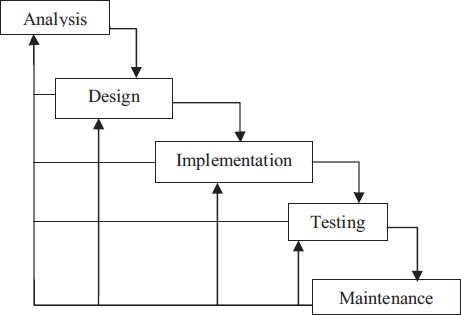
\includegraphics[width=0.60\linewidth]{iterative-waterfall.png}
	\captionof{figure}{\textit{Typical iterative Waterfall methodology }}
	\label{fig:iterativewaterfall}
\end{figure}

This change in methodology was deemed to be necessary, as it felt more appropriate for the project as a whole when compared to agile and waterfall separately.

% Agile
% methodologies, while fitting for any software project, puts a focus on constant customer feedback during the SDLC , 
% something that there would be a lack of in this project's case. The Waterfall methodology, while a lot simpler to plan with, its lack of flexibility when it comes to changes 
% in project scope and lack of prototype creation in particular , made it usage unfitting for the project. 

Combining parts 
of these methodologies however, made for a methodology that was fitting for the project as a whole. 

% Though this was a unforeseen risk according to the risk matrix and risk 
% register composed before the beginning of development (see Appendix B), 

this change did not negatively affect development, despite this shift occurring slightly into the 
execution of the project, 

% as the project was able to stick to its defined timeline throughout the duration of the project execution (see Appendix C). \newline

The Hybrid model was used by using a waterfall approach for the Requirements Analysis, Design, and Evaluation stage, and combining it with an iterative approach for the 
Implementation and Testing stage. The requirements were defined during the beginning of the project's execution stage within a Software Design Specification 
(see Appendix F), then, based on the requirements specified, designs surrounding those requirements were created.

\begin{figure}[H]
\centering
	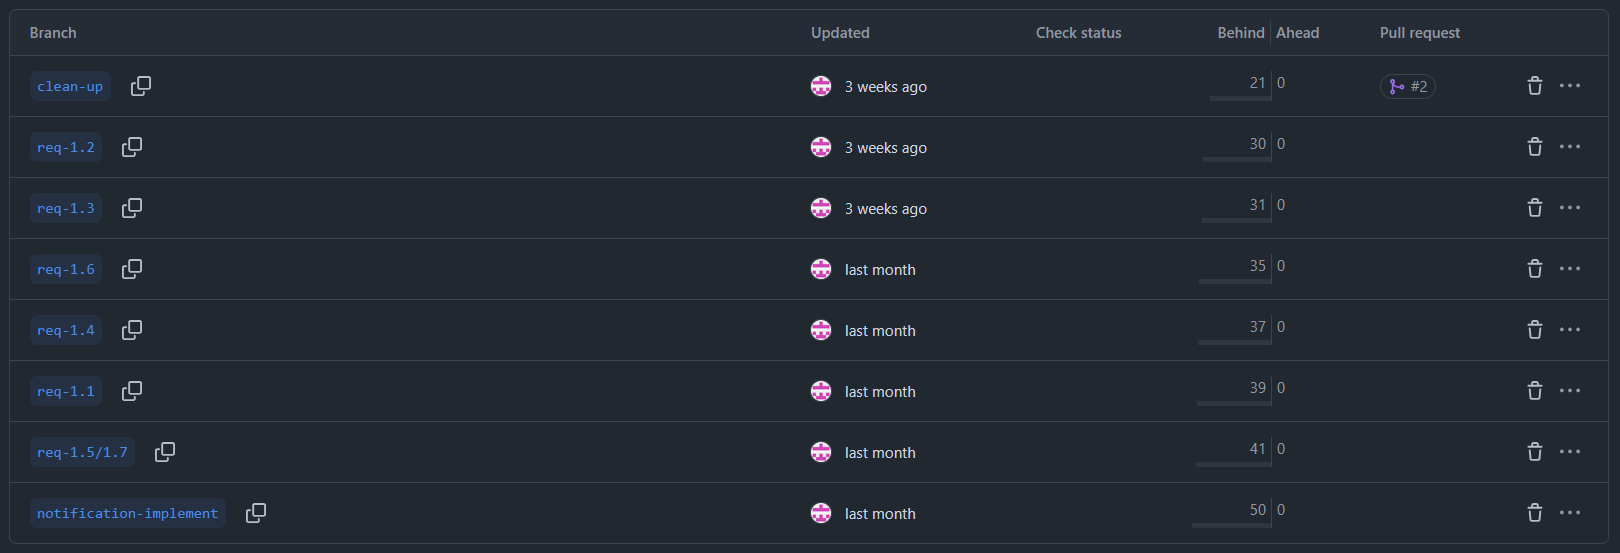
\includegraphics[width=1\linewidth]{git-branches.png}
	\captionof{figure}{\textit{GitHub branches for each requirement}}
	\label{fig:gitbranch}
\end{figure}

Figure \ref{fig:gitbranch} showcases the process behind implementing and testing the PRI. 

% A GitHub branch that matched the name of the requirement was 
% created, then, within that branch, that requirement was implemented, then tested upon via Incremental Integration Testing to ensure the requirement was implemented as intended. 

If that 
part of the requirement passed all test cases, a new GitHub branch for the next requirement was created using the newly completed requirement as a blueprint, and this process 
repeated until the implementation of all requirements were completed.

\newpage

\subsection{Requirements Analysis}
When performing the requirements analysis for the project, the research statement as stated in section 1.2.1 was analysed to identify the main components of the application. Combining this with
the knowledge gained after performing the literature review provided the blueprint from where functional (and non-functional) requirements could be identified. As a reminder, the research
statement was:\newline

\textit{To create a mobile application that integrates psychological intervention methods alongside usage tracking technologies to help address smartphone and social media addiction}\newline

From the research statement alone, two integral components can be identified:

\begin{enumerate}
	\item A psychological intervention method that can be integrated into a mobile application
	\item A code-based technical method of tracking smartphone and social media usage
\end{enumerate}

From here, these components can then be broken down into smaller parts that then make up a list of functional requirements after ensuring they fit within the findings of the literature
review, 

% with some aspects from both components being used to identify a requirement. 

Additionally, interviews were conducted with nine participants to help identify new requirements or 
to add pieces to existing requirements. 
Interview details can be found within Appendices D and E. \newline

\subsubsection{Psychological Intervention Method}

% The psychological intervention method is a critical component for the PRI, as this would then ben used to derive functional requirements of the application, therefore,
Choosing a psychological intervention method came down to how easy it would be to integrate said method into a mobile app and how impactful the method itself is when used. The literature review,
specifically section 2.3 made mention of two psychological intervention methods, Cognitive Behavioural Therapy and Reality Therapy. \newline

After analysing both frameworks, it was concluded that RT was the choice of framework to use. The primary reason for using this framework instead of CBT ties back to one of the main criticisms
of SA \& SMA mobile apps found within the literature review, that being that current apps on the market do not provide any opportunity for end-users to be made aware of their usage or SA \& SMA
as a whole. RT's framework inherently gives a person the opportunity to understand what's stopping them from achieving their goal, where in this
case, their smartphone usage and/or SA \& SMA would be the aspect affecting them. Meanwhile, CBT in its framework doesn't inherently provide this opportunity. \newline

\subsubsection{Usage Tracking Method}

% Finding a usage tracking method was a simple task. 

As mentioned in section 2.4, Apple's iOS operating system disallows apps from tracking a user's usage
due to privacy concerns, with the only "viable" alternative being using a "jailbroken" device, which would complicate multiple parts of the project. On the contrary, Google's Android operating system
allows for apps to track a user's usage via the "android.app.usage" package within its API, so long that a user permits the app to do so.

\begin{figure}[H]
\centering
	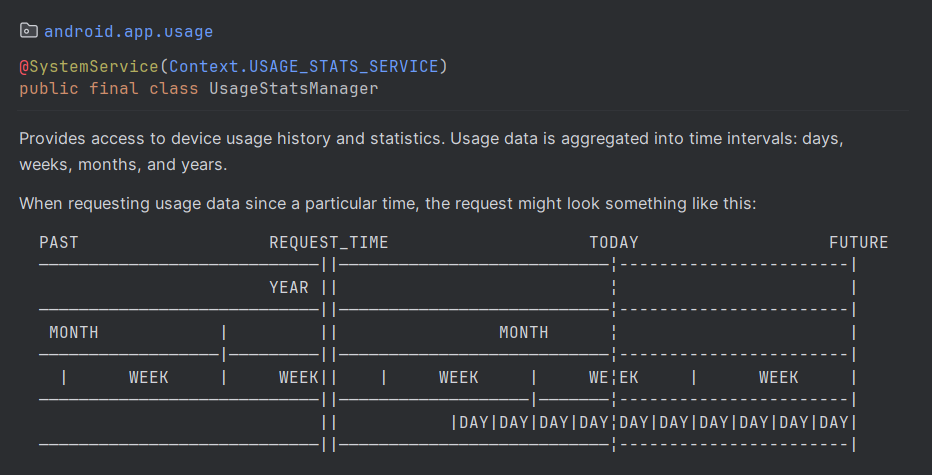
\includegraphics[width=1\linewidth]{usagestatsmanager-api-doc.png}
	\captionof{figure}{\textit{UsageStatsManager class from android.app.usage, taken from Android's API documentation within Android Studio }}
	\label{fig:usagestatsmanager}
\end{figure}

The "android.app.usage" package contains many classes that provide detailed statistics about a user's device, namely the "UsageStatsManager" 
class. Figure \ref{fig:usagestatsmanager} shows how this class returns a request for usage data, with the documentation noting that requesting usage data within a time interval will include that
interval. This class was mentioned within the literature review when discussing what methods could 
be used to track usage of a user's device, and is the class of choice for developing the app, as it contains a method "queryUsageStats" that can be used to retrieve usage stats within a specified 
time range .

\subsubsection{Functional (and Non-Functional) Requirements}

As mentioned at the beginning of this section, requirements were identified by taking the findings from the literature review and combining them alongside the analysis of the research statement and
user interviews that were performed as well. All requirements were then compiled into a Software Requirements Specification document.

\begin{table}[H]
\centering
\resizebox{\textwidth}{!}{%
\begin{tabular}{@{}l|l@{}}
\toprule
\textbf{REQ-1.5}             &                                                                                                                                                                                                                                                                   \\ \midrule
\textbf{Description}         & \begin{tabular}[c]{@{}l@{}}When launching the app for the first time, guide the user by providing information \\ on SM and SMA, helping the user set up a goal, and suggesting alternative activities to \\ partake in.\end{tabular}                              \\ \cmidrule(l){2-2} 
\textbf{Software Input}      & User launches the application for the first time, also includes textual user inputs when setting goals                                                                                                                                                            \\ \cmidrule(l){2-2} 
\textbf{Software Processing} & \begin{tabular}[c]{@{}l@{}}Take the user inputted goal, and set it as the current goal until it is manually updated \\ by the user, as well as any alternative activities the user can come up with\end{tabular}                                                  \\ \cmidrule(l){2-2} 
\textbf{Software Output}     & \begin{tabular}[c]{@{}l@{}}Display a brief overview of the purpose of the app, alongside prompts for user input \\ such as goals, and a user's own activity suggestions. Upon completion, display the main \\ view of the app (see functional requirement 1.1)\end{tabular} \\ \cmidrule(l){2-2} 
\textbf{Other}               & N/A                                                                                                                                                                                                                                                               \\ \cmidrule(l){2-2} 
\textbf{Constraints}         & User must not have completed the onboarding process / User must have never ran the app before                                                                                                                                                                     \\ \cmidrule(l){2-2} 
\textbf{Data Handling}       & \begin{tabular}[c]{@{}l@{}}Similar to functional requirement 1.4, handle user input by restricting the character \\ limit to a pre-determined amount\end{tabular}                                                                                                     \\ \cmidrule(l){2-2} 
\textbf{Error Handling}      & \begin{tabular}[c]{@{}l@{}}If the user closes the app during the onboarding phase, reset the onboarding phases to the \\ first step; similar to if the user had opened the app for the first time again\end{tabular}                                              \\ \bottomrule
\end{tabular}%
}
\caption{Functional Requirement 1.5}
\label{tab:func-req-1-5-main}
\end{table}

Table  \ref{tab:func-req-1-5-main} shows an example of how a requirement was defined within the SRS. It contains a description of how it would function normally, the inputs required from an end-user
to ensure its functionality, the processing required by the application, the output the app should show to an end-user after processing, constraints of the requirement, how the app should handle
any data used for the requirement, and how the app should handle errors the requirement may be prone to.

\begin{table}[H]
\centering
\resizebox{\textwidth}{!}{%
\begin{tabular}{@{}l|ll@{}}
\toprule
\textbf{Req. ID} & \textbf{Requirement Name}                                                                                                        & \textbf{Requirement Description}                                                                                                                                                                                                           \\ \midrule
\textbf{REQ-1.1} & View overall application usage                                                                                                   & \begin{tabular}[c]{@{}l@{}}Allow the user to access a visual \\ graph showcasing their app usage over \\ the past week\end{tabular}                                                                                                        \\ \cmidrule(l){2-3} 
\textbf{REQ-1.2} & \begin{tabular}[c]{@{}l@{}}Compare app usage from one \\ week to the last\end{tabular}                                           & \begin{tabular}[c]{@{}l@{}}Allow the user to compare their \\ app usage stats from one week to \\ another, with the function also giving \\ a percentage of the usage increase or decrease\end{tabular}                                    \\ \cmidrule(l){2-3} 
\textbf{REQ-1.3} & \begin{tabular}[c]{@{}l@{}}Give guidance based on RT to the user \\ if overall app usage is higher than last week’s\end{tabular} & \begin{tabular}[c]{@{}l@{}}If a user has seen a substantial increase in app \\ usage from one week to another, provide step-by-step \\ guidance to the user, similar to that seen when\\ launching the app for the first time\end{tabular} \\ \cmidrule(l){2-3} 
\textbf{REQ-1.4} & Update current goal                                                                                                              & \begin{tabular}[c]{@{}l@{}}Allow the user to update their current goal, originally \\ defined when launching the app for the first time\end{tabular}                                                                                       \\ \cmidrule(l){2-3} 
\textbf{REQ-1.5} & \begin{tabular}[c]{@{}l@{}}Guide the user through setting up \\ the app for continued use\end{tabular}                           & \begin{tabular}[c]{@{}l@{}}When launching the app for the first time, guide the \\ user by providing information on SM and SMA, helping \\ the user set up a goal, and suggesting alternative \\ activities to partake in\end{tabular}     \\ \cmidrule(l){2-3} 
\textbf{REQ-1.6} & \begin{tabular}[c]{@{}l@{}}Send current usage statistics for \\ future analysis\end{tabular}                                     & \begin{tabular}[c]{@{}l@{}}Allow the user to send their current usage statistics to \\ the project leader for analysis and evaluation\end{tabular}                                                                                         \\ \cmidrule(l){2-3} 
\textbf{REQ-1.7} & Suggest alternative activities                                                                                                   & \begin{tabular}[c]{@{}l@{}}Provide the user with alternative activities to do \\ instead of using their smartphone / social media\end{tabular}                                                                                             \\ \cmidrule(l){2-3} 
\textbf{REQ-1.8} & Update current set of activities                                                                                                 & \begin{tabular}[c]{@{}l@{}}Allow the user to update their current set of activities \\ originally defined when launching the app for the first time.\end{tabular}                                                                          \\ \bottomrule
\end{tabular}%
}
\caption{Functional Requirements Master List}
\label{tab:func-req-master-list}
\end{table}

%possibly shorten - move to appendix
Table \ref{tab:func-req-master-list} provides a full list of all the functional requirements identified throughout the project's lifespan. 

% With the exception of "REQ-1.8", where the requirement
% was identified and defined later during development, all requirements were identified during the initial requirements analysis phase of development. 

A comprehensive breakdown of each functional 
requirement identified in detail, similar in manner to Table \ref{tab:func-req-1-5-main}, alongside non-functional requirements can be found in Appendix F, as well as the SRS document separately 
via the GitHub repository.


\newpage

\subsection{Design}
The next step was to design both design diagrams that represent how the requirement should typically function for an 
end-user and user interfaces for each screen necessary per requirement. 

% below text wall probably unnecessary

% Before performing this step, a decision had to made on if the design diagrams for each requirement should be created first
% before creating the user interfaces, or if each design diagram and UI should be created on a "per-requirement" basis. Ultimately, it was decided to create diagrams for each requirement first, as
% when it came time to work on the interfaces, the author would have the best understanding possible up to that point on how parts of the application would interact with each other, and therefore would
% have a better understanding on what UI elements would be included. \newline

\subsubsection{Diagram Design}

The type of diagram used for designing the application based on the requirements was a Flowchart diagram, a diagram which uses components, typically shapes, that represent logic, order, and decision-points within a system
to model said system or related processes, making it easy for developers to understand event sequences or the overall structure of a system .

% This type 
% of diagram was decided upon due to how easily it can convey the idea of how a requirement should function . Flowchart diagrams were the 
% exclusive diagram used for designing the application.

\begin{figure}[H]
\centering
	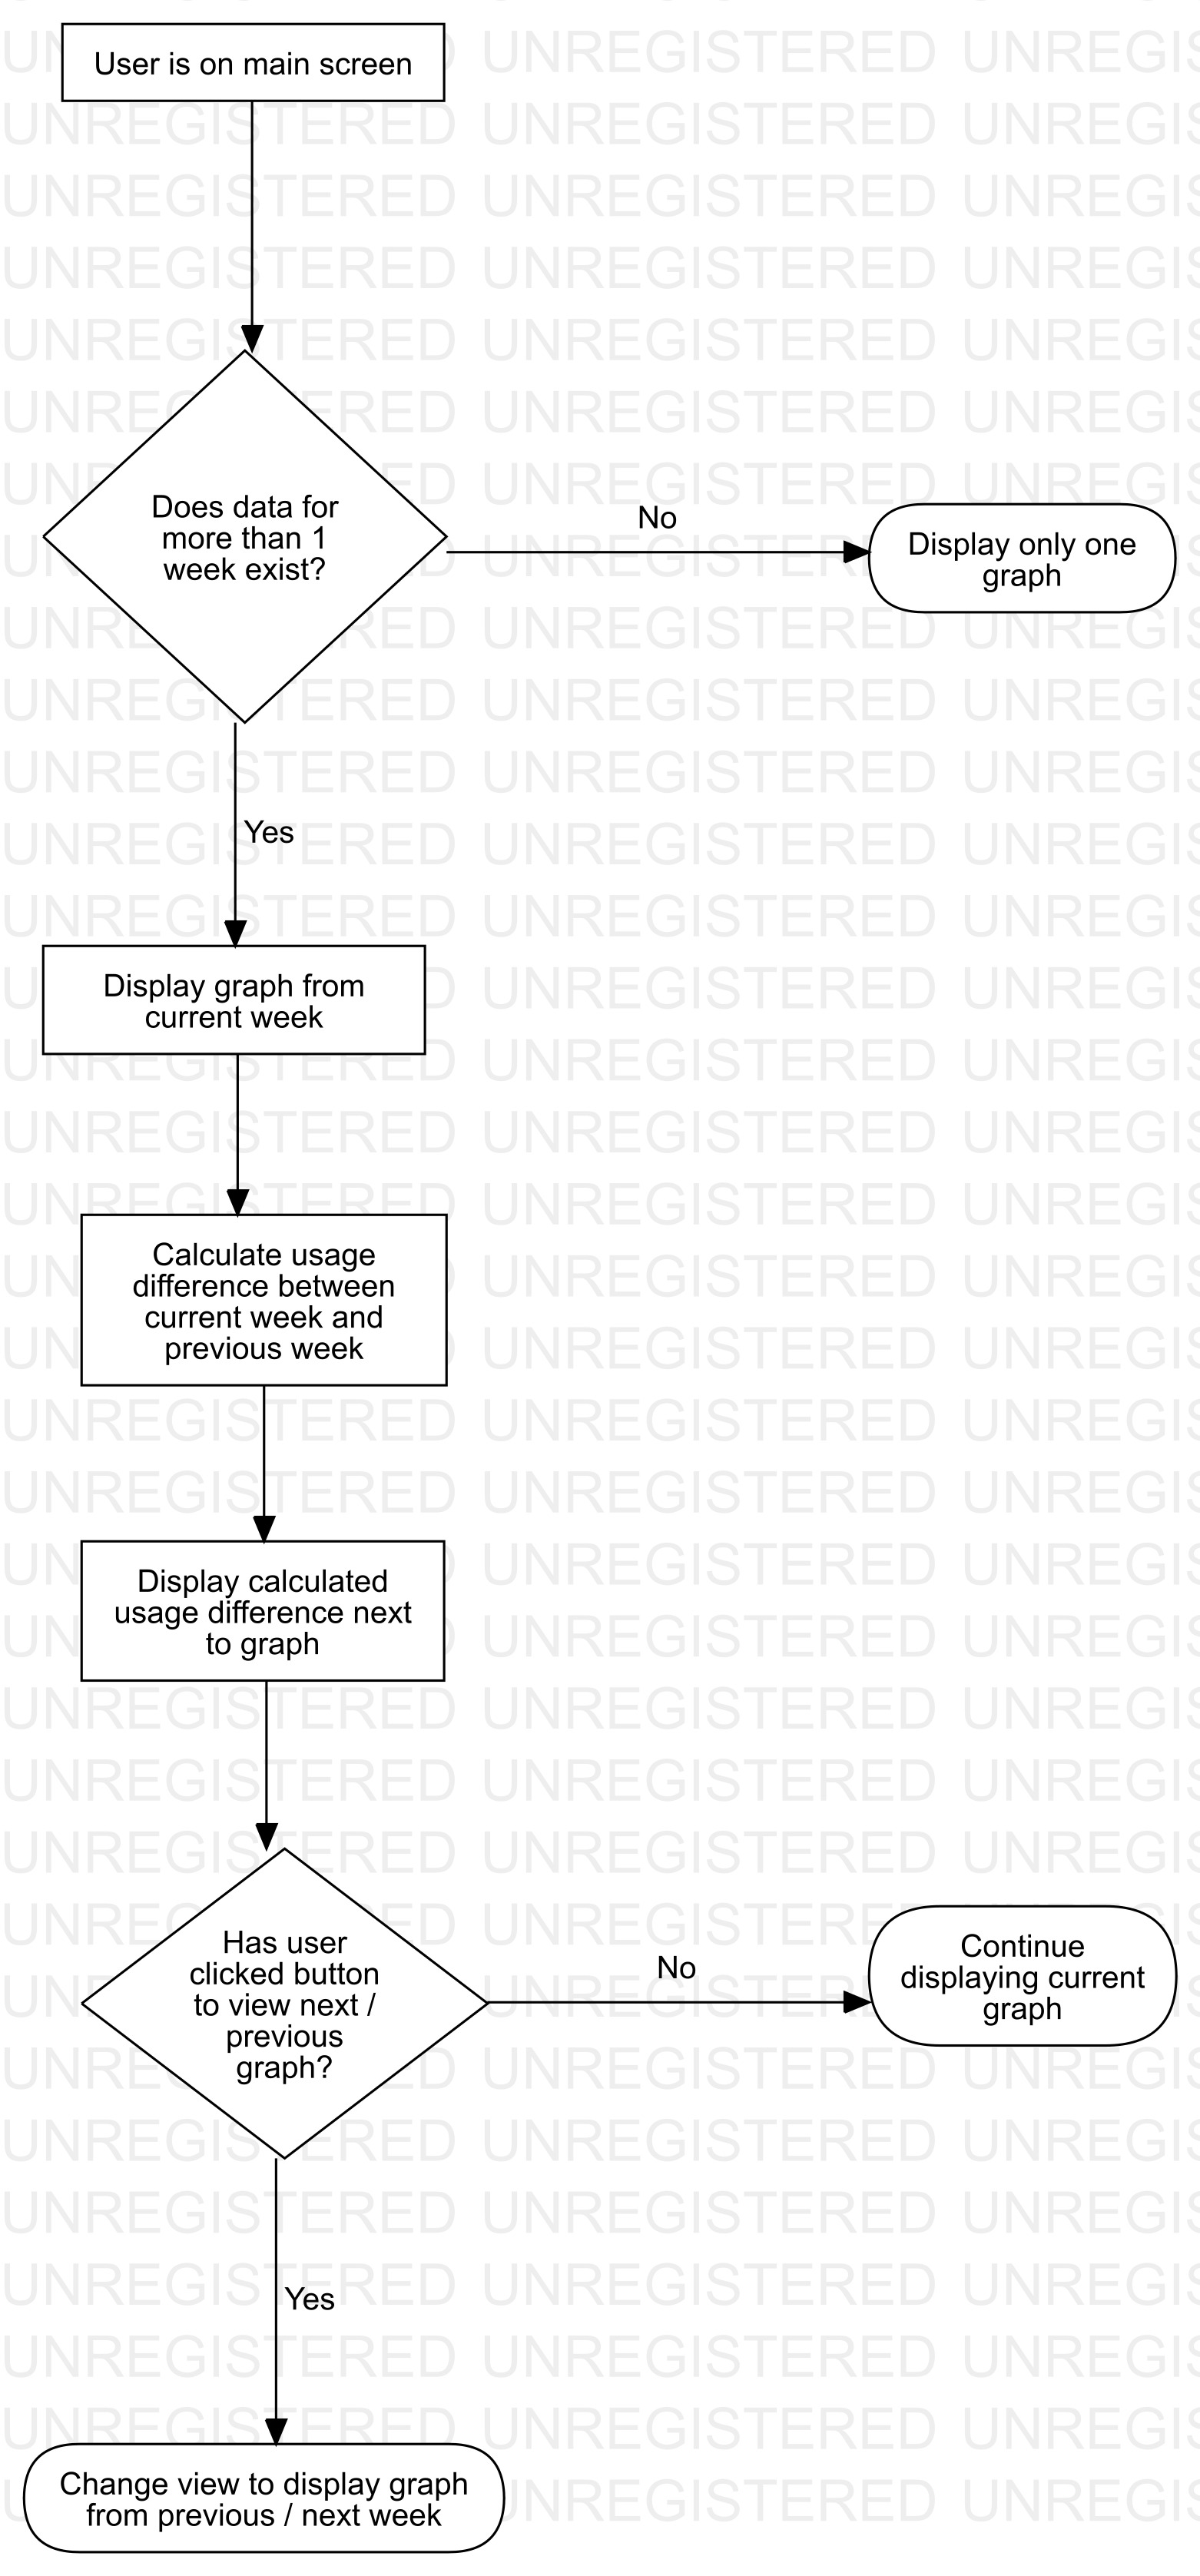
\includegraphics[width=0.45\linewidth]{example-flow-chart-req-1_2.jpg}
	\captionof{figure}{\textit{Req-1.2 Flowchart Diagram}}
	\label{fig:req1-2-flowchart-diagram}
\end{figure}

Figure \ref{fig:req1-2-flowchart-diagram} provides an example of the flowchart diagrams created during the design stage. The oval shapes represents the start and end points for a diagram, the arrow 
lines represent the path taken by the program during execution, the diamond shapes represent decisions that are to be made by the app, and the rectangles represent processes during the execution 
of the app. Typically, more shapes are used to represent other parts of a system design, however, to keep the design as simple possible to understand, the prior three shapes were the only ones 
utilised during this process, with the level of complexity in the designs varying depending on if elements such as error handling were part of the requirement. \newline

% As mentioned at the beginning of this section, 

This process of creating a flowchart based on the requirement was repeated until all requirements outlined had a flowchart diagram. From there, the designs
were reviewed for any possible refinements, for which only one flowchart needed refinement, that being requirement 1.3. 

% Requirements were created in sequential order according to the requirement number 
% (Req-1.1 $\rightarrow$ Req-1.2 $\rightarrow$ Req-1.3 $\rightarrow$ etc\dots). 

A complete list of the flowchart diagrams created can be found in Appendix G.

\begin{figure}[H]
\centering
	\centering
	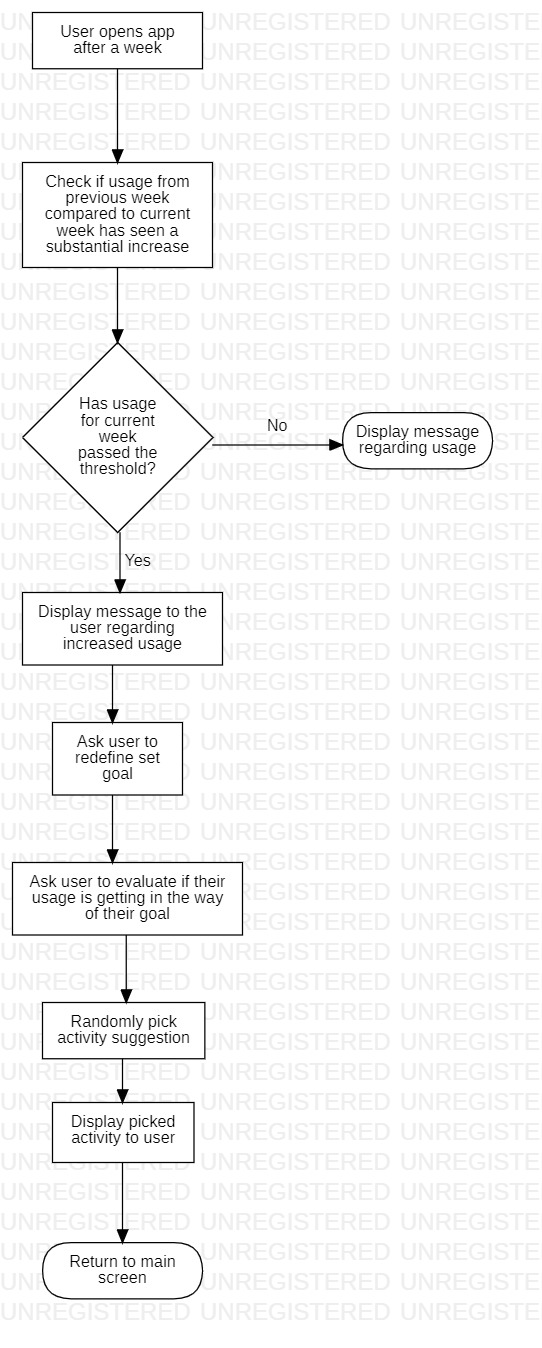
\includegraphics[width=0.40\linewidth]{diagrams/req-1.3-diagram-old.jpg}
	\captionof{figure}{\textit{First iteration of requirement 1.3's flowchart design}}
	\label{fig:req-1_3-old}
\end{figure}


\begin{figure}[H]
	\centering
	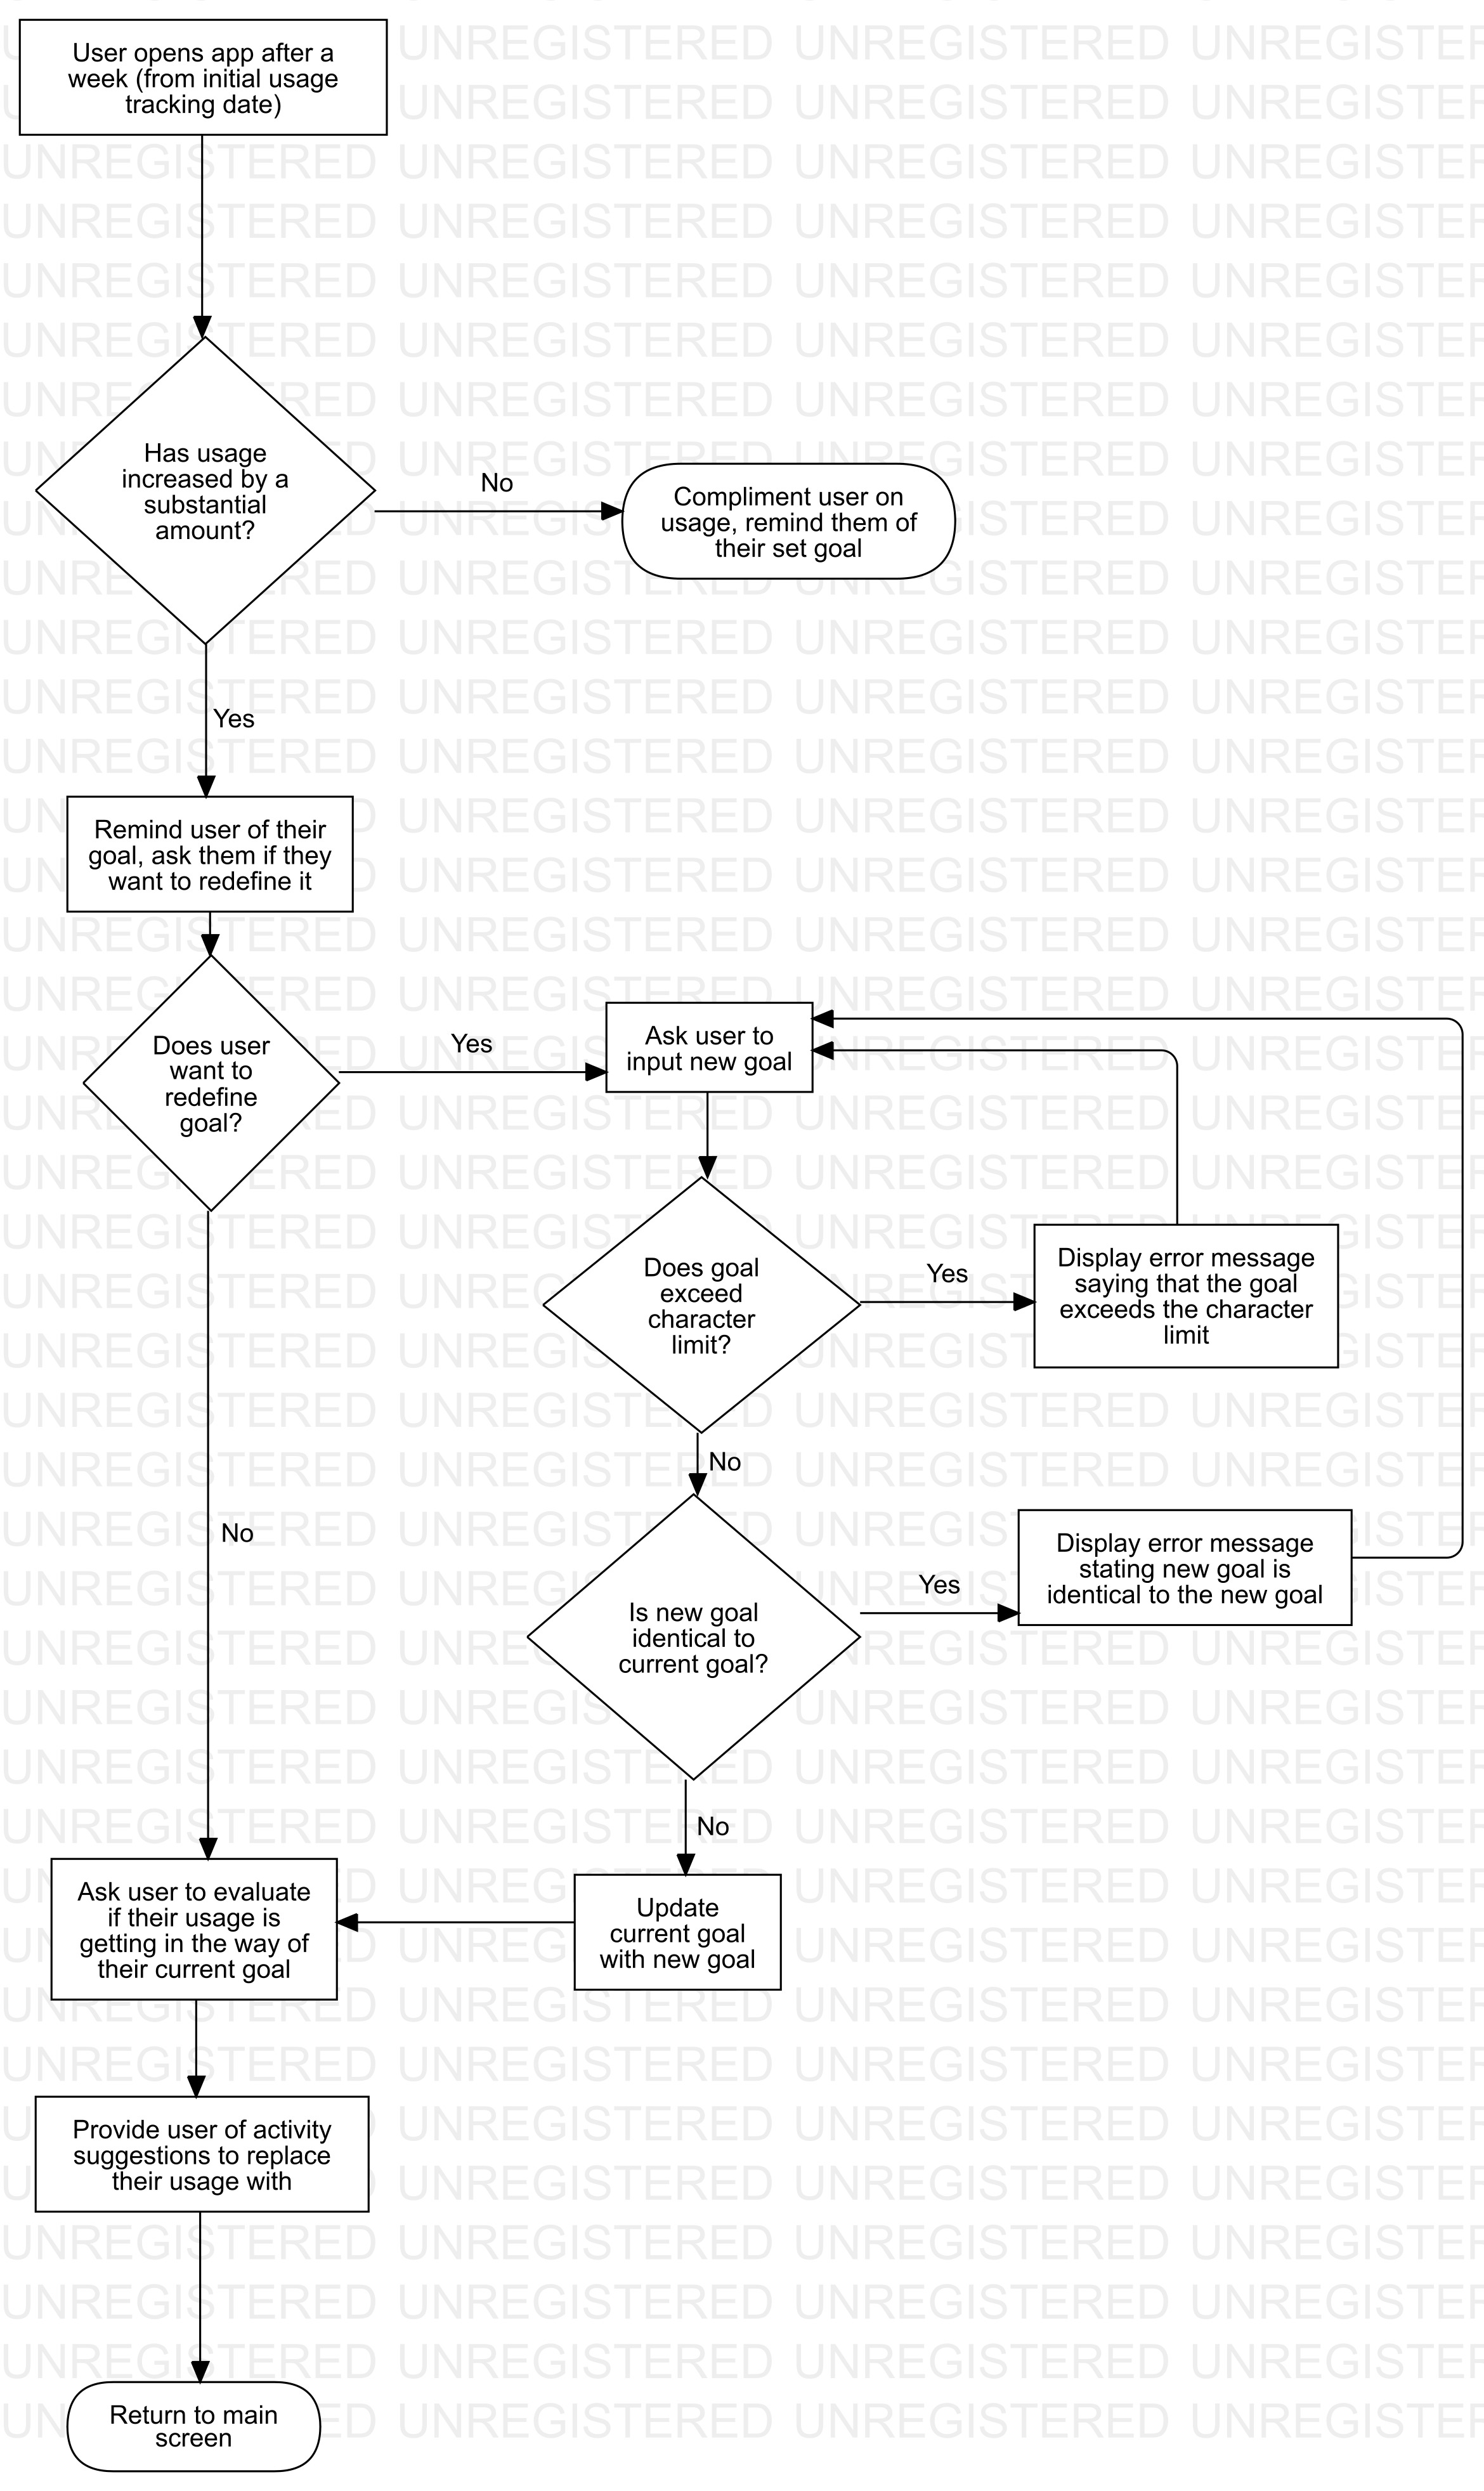
\includegraphics[width=0.45\linewidth]{diagrams/req-1_3-diagram.jpg}
	\captionof{figure}{\textit{Final iteration of requirement 1.3's flowchart design}}
	\label{fig:req-1_3-new}
\end{figure}

Figures \ref{fig:req-1_3-old} and \ref{fig:req-1_3-new} show the first and last iterations respectively of the flowchart design for requirement 1.3. 

% While the design for the requirement is the same, 

The 
later iteration shows greater detail, providing more decision-points and error handling in the scenario the user wants to redefine their goal, while also making some changes to the wording of the process points.

\begin{figure}[H]
\centering
	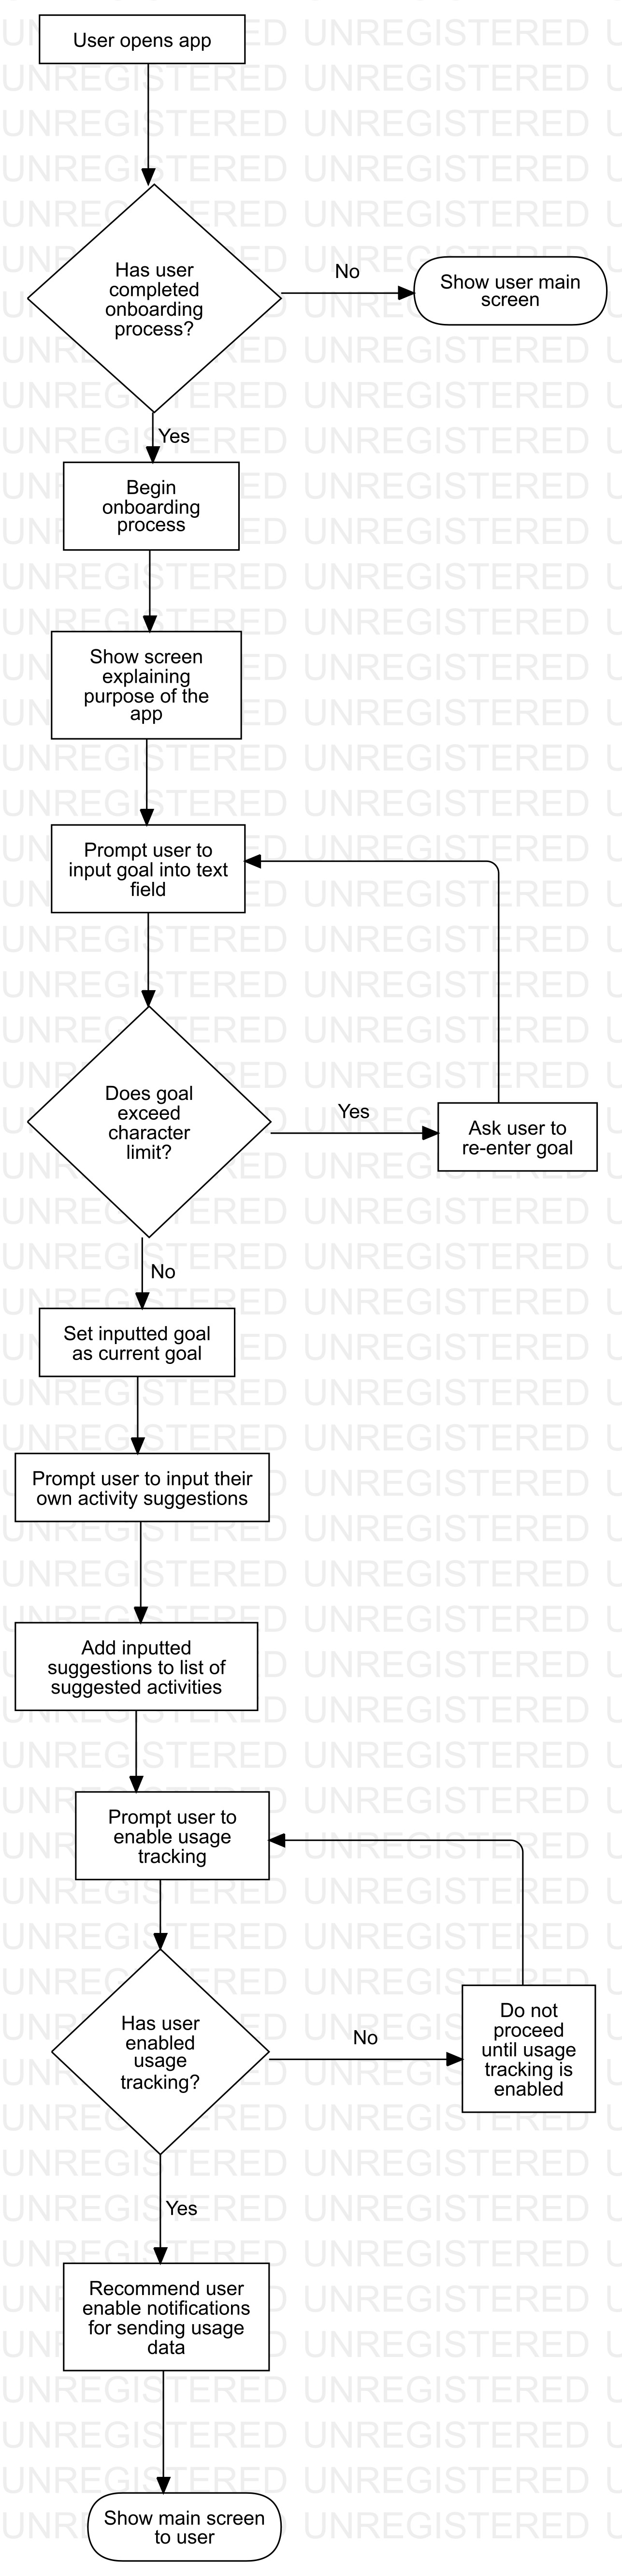
\includegraphics[width=0.32\linewidth]{diagrams/req-1_5__1_7-diagram.jpg}
	\captionof{figure}[]{\textit{Req-1.5 / Req-1.7 Flowchart Diagram}}
	\label{fig:req1-5-7-diagram-main}
\end{figure}

Figure \ref{fig:req1-5-7-diagram-main} shows the flowchart diagram of requirements 1.5 and 1.7, merged into a single requirement. When creating both requirements, it was identified that requirement 1.7 could
only function if the app was at a specific point (See Appendix F). 

% Requirement 1.7's constraints notes that: \newline

% \textit{"User must be currently given guidance by the app, or is in the onboarding section of the app"}\newline

This means that the requirement can't be met unless the app is in the onboarding stage (outlined in requirement 1.5) or is currently providing guidance to the user (outlined in requirement 1.3). To avoid 
replication when creating the flowcharts, requirements 1.5 and 1.7 were merged into a single diagram. 

%While including requirement 1.3 within the merge was considered, requirement 1.3 was left out of the merge, due
%to the general flow being different enough to deem it unique, especially after it's aforementioned redesign.


\subsubsection{User Interface Design}
When designing the UI, a wireframing approach was used. This approach involves creating simplistic designs of an interface to establish structure and design flow.

% Wireframe designs are meant to be basic in terms of visual spectacle, acting as a blueprint for a user interface, and keeping its focus solely on fundamental design elements such as where important
% parts of a UI should go . 

The intention from the start was to keep the UI as simple as possible, ensuring that an end-user wasn't overwhelmed from using the app while
making sure all essential elements for the interface were included, therefore, this approach was deemed to be the most effective way of creating the UI.\newline

The wireframes created for the UI consist of "Mid-Fidelity" wireframes, which can be defined as a compromise between "Low-Fidelity" and "High-Fidelity" wireframes, providing clearer structure of an
interface while making use of little to no visual flair or colouring. 

% While all three types of wireframing would be included in the UI design stage
% of a typical SDLC, making exclusive use of Mid-Fidelity wireframes meant less time was spent creating many different types of wireframes, and more time was spent delivering and perfecting a simpler and 
% easy-to-implement UI design.\newline

Because all of the requirements had already been established (with the exception of requirement 1.8), there was a fairly clear understanding of what UI elements needed to be included to ensure 
functionality for each requirement. One screen by itself did not meet the functionality for each requirement, meaning the creation of multiple screens were necessary to ensure each requirement was
met. 

% Concerning how the screens needed for each requirement should be ordered, the flowcharts established how the screens should be ordered.

\begin{figure}[H]
\centering
	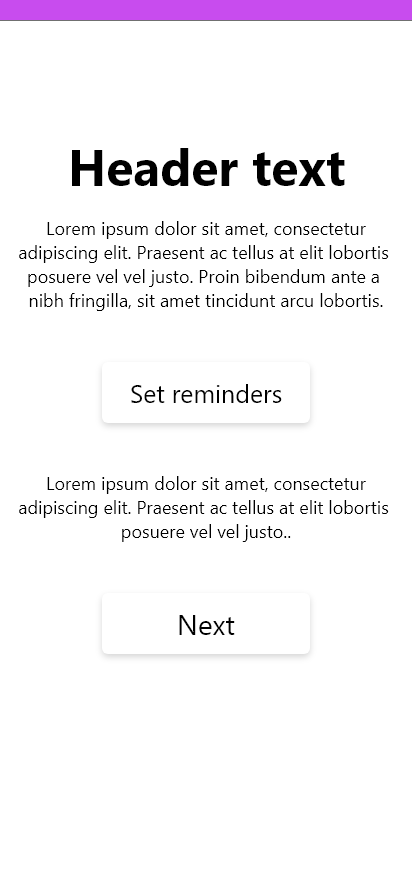
\includegraphics[width=0.45\linewidth]{ui/Onboarding Notification Screen.png}
	\captionof{figure}{\textit{UI wireframe of the "Enable Notifications" screen during the onboarding process - Made for Requirement 1.5/1.7}}
	\label{fig:ui-wireframe-example}
\end{figure}

An example of the UI interface design created can be seen in figure \ref{fig:ui-wireframe-example}. The UI in this example seen showcases three core elements, the "Header Text" in large, bold text, denoting
the heading for that screen, smaller text shown by the "Lorem ipsum" text, used for communication information to a user, and a button shown by the rectangle with the drop-shadow, denoting interactive
elements for the screen. A full list of the screens created can be found in Appendix H.\newline

\begin{figure}[H]
\centering
	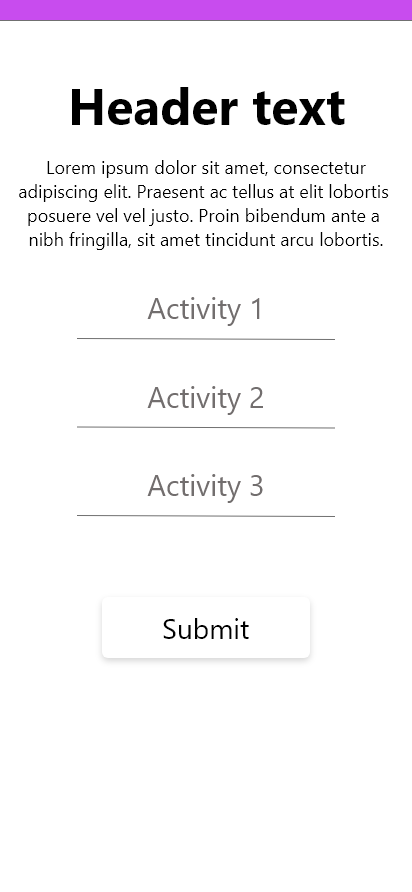
\includegraphics[width=0.45\linewidth]{ui/Onboarding Activity Entry Screen.png}
	\captionof{figure}{\textit{UI wireframe of the "Activity Entry Screen" screen during the onboarding process - Made for Requirement 1.5/1.7}}
	\label{fig:ui-wireframe-activity-entry-main}
\end{figure}

\begin{figure}[H]
\centering
	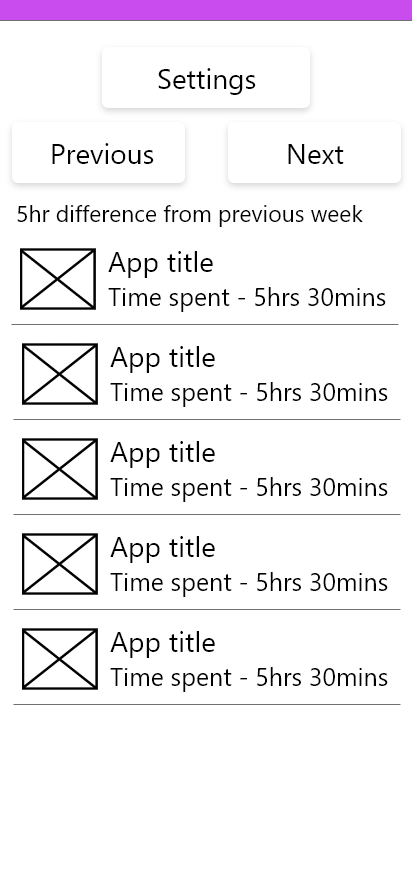
\includegraphics[width=0.45\linewidth]{ui/Main Screen.png}
	\captionof{figure}{\textit{UI wireframe of the Main Screen}}
	\label{fig:ui-wireframe-main-screen}
\end{figure}

Each screen was varied in terms of interactive elements, text required, etc. Figures \ref{fig:ui-wireframe-activity-entry-main} and \ref{fig:ui-wireframe-main-screen} show examples of different elements
that a screen may include, such as lists or text entry fields. 

% Figure \ref{fig:ui-wireframe-activity-entry-main} adds input fields, shown by the lighter coloured text with the line underneath, while figure \ref{fig:ui-wireframe-main-screen}
% removes the header text element and adds a list. The list itself contain other elements, notably an image, alongside text stacked on top of each other. \newline

While creating these screens, it was also determined that some of the screens can be reused in other requirements. For example, the screen used for entering a goal are needed in requirements 1.4 and
1.5, meaning time could be saved from not having to create another screen.

\newpage

\subsection{Implementation}
% As noted previously in section 3.3, this part of the project, alongside the testing part of the project, made use of an iterative approach. 

At this stage, implementing the project would consist
of using the information gathered during the requirements analysis stage, then taking the flowchart diagrams and UI wireframes created from the design stage, and implementing
them according to the documentation.

% Implementing each requirement facilitated backend development via implementing the functionality for the requirement and frontend development via implementing
% the user interface the end-user would interact with. Therefore, the primary type of development executed can be considered full-stack. \newline

Figure \ref{fig:gitbranch} from section 3.3 provides the implication, however, it should be plainly stated that the requirements weren't implemented in sequential order, as the author found that it
would prove troublesome attempting to implement some requirements before others 

% (e.g. trying to implement functionality to allow a user to update a goal (Req-1.4) before functionality for setting
% a goal has been implemented (Req-1.5)). 

Rather, requirements were implemented in an order of what would be feasible to implement at that point in development.

\subsubsection{Proof-of-Concept Prototype(s)}
Before beginning work on any of the requirements, a subfolder that would contain a basic prototype for ensuring the UsageStatsManager class discussed in section 2.4 can 
return the data necessary for the app to function as intended and ensuring the app's notification system was created. This would serve as a blueprint from where the app would then be built upon. 

% Backend development was the primary type of development carried out at this point.

\begin{lstlisting}[language=Java, style=mystyle, caption={loadUsage() function}, label=lst:loadUsage]
public void loadUsage() throws PackageManager.NameNotFoundException {
	long lastWeek = System.currentTimeMillis() - (1000*3600*24*7);
	UsageStatsManager usm = (UsageStatsManager)this.getSystemService(USAGE_STATS_SERVICE);
	List<UsageStats> appList = usm.queryUsageStats(UsageStatsManager.INTERVAL_WEEKLY,
			lastWeek, System.currentTimeMillis());
	appList = appList.stream().filter(app -> app.getTotalTimeInForeground() > 0).collect(Collectors.toList());

	Log.d("usagestats", appList.toString());

	if (!appList.isEmpty()) {
		Map<String, UsageStats> sortedMap = new TreeMap();
		for (UsageStats usageStats : appList) {
			sortedMap.put(usageStats.getPackageName(), usageStats);
		}
		Log.d("moreStats", sortedMap.toString());
		showUsage(sortedMap);
	}

}
\end{lstlisting}

Code snippet \ref{lst:loadUsage} shows the function used to fetch the usage data for the user. This function is called on app startup.

% as it gets called within the onCreate method. 

The function calls the
"queryUsageStats" method from the UsageStatsManager class to get the usage stats from the last week, then stores it in a list, then, if the list isn't empty, maps it to a tree map then calls 
another function "showUsage" to show the usage to the user. Some of the code seen above was sourced from an external sample project, see Appendix I for more information. \newline

After ensuring that all the necessary information was able to be fetched from the UsageStatsManager class, a separate folder was created that focused on fully developing the app. The folder
structure can be seen below in figure \ref{fig:folder-structure}.

\begin{figure}[H]
\centering
	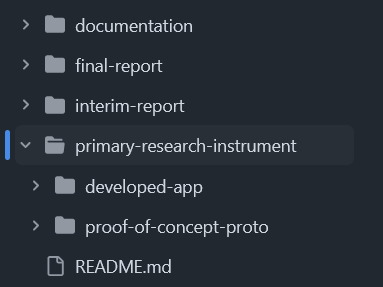
\includegraphics[width=0.45\linewidth]{folder-structure.png}
	\captionof{figure}{\textit{Folder structure of GitHub repo}}
	\label{fig:folder-structure}
\end{figure}

This is where a secondary prototype was created, used for ensuring the app was able to send notifications reminding the user to send their usage statistics was able to be implemented. As the 
evaluation involved testing the application with human participants, implementing a reminder system using notifications was thought to be a necessary feature to ensure the data is sent in a timely manner. 

% To 
% achieve this, implementing notifications was the idea decided upon.

\begin{lstlisting}[language=Java, style=mystyle, caption={PeriodicWorkRequest class used for sending notifications}, label=lst:periodicworkrequest]
final PeriodicWorkRequest periodicWorkRequest =
		new PeriodicWorkRequest.Builder(WorkerClass.class, 5, TimeUnit.SECONDS, 15, TimeUnit.MINUTES)
		.addTag("periodicWork")
		.build();

notiTestBtn.setOnClickListener(view ->
		WorkManager.getInstance().enqueue(periodicWorkRequest));
\end{lstlisting}

\begin{lstlisting}[language=Java, style=mystyle, caption={WorkerClass class used for sending notifications}, label=lst:workerclass]
public class WorkerClass extends Worker {

    public WorkerClass(@NonNull Context context, @NonNull WorkerParameters workerParams) {
        super(context, workerParams);
    }

    @NonNull
    @Override
    public Result doWork() {
        try {
            Thread.sleep(1000);
        } catch (InterruptedException e) {
            e.printStackTrace();
        }

        sendNoti();

        return Result.success();
    }
    public void sendNoti() {
        NotificationManager notiManager = (NotificationManager)getApplicationContext().getSystemService(Context.NOTIFICATION_SERVICE);
        if (Build.VERSION.SDK_INT >= Build.VERSION_CODES.O) {
            CharSequence name = "FocusathChannel";
            String desc = "App notification channel for Focusath";
            int importance = NotificationManager.IMPORTANCE_DEFAULT;
            NotificationChannel channel = new NotificationChannel("default", name, importance);
            channel.setDescription(desc);
            //NotificationManager notificationManager = getSystemService(NotificationManager.class);
            notiManager.createNotificationChannel(channel);
        }

        NotificationCompat.Builder notification = new NotificationCompat.Builder(getApplicationContext(), "default")
                .setContentTitle("title")
                .setContentText("message")
                .setSmallIcon(R.mipmap.ic_launcher);
        notiManager.notify(1, notification.build());
    }

}

\end{lstlisting}

Code snippet \ref{lst:periodicworkrequest} and \ref{lst:workerclass} shows the code and class used for sending notifications. It defines a PeriodicWorkRequest variable
that triggers the code in code \ref{lst:workerclass} every 5 seconds, 15 minutes or later from the last trigger, then, creates an OnClickListener that queues the PeriodicWorkRequest. Code snippet
\ref{lst:workerclass} executes the doWork() method which calls sendNoti() function. This builds the notification to be sent to the user, before displaying it to the user. Seeing as the code in both 
snippets were for ensuring functionality, both would be refined over the course of development. 

% Note that code snippet \ref{lst:periodicworkrequest} would later be changed to trigger every 7 days, and
% the current trigger time was in place for testing and debugging.\newline

This prototype would also establish the class structure for the app, as can be seen in figure \ref{fig:class-structure} below. By the end of development, RecyclerViewAdapter would be the only class
removed.

\begin{figure}[H]
\centering
	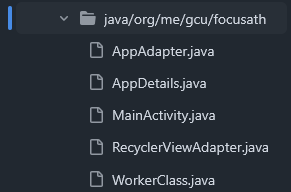
\includegraphics[width=0.45\linewidth]{class-structure.png}
	\captionof{figure}{\textit{Class structure of PRI at the prototyping stage}}
	\label{fig:class-structure}
\end{figure}

\subsubsection{Req-1.5 / 1.7} %make sure to highlight stuff mentioned in requirements
This branch focused on creating the onboarding process, the process the user goes through when opening the app for the first time, and expands on the groundwork established with the previous
prototype. Development with regards to the SRS began with these requirements as this would establish the core functionality of the app. 

% so building from this point onwards was thought to be the 
% easiest.

\begin{lstlisting}[language=Java, style=mystyle, caption={Checks if user has completed onboarding process}, label=lst:isOnboardingCompleteCheck]
isOnboardingComplete = sharedPreferencesOnBoarding.getBoolean("isOnboardingComplete", false);
	if (!isOnboardingComplete) {
		if (screen_count > 1) {
			sharedPreferencesOnBoarding.edit().putBoolean("isOnboardingComplete", false).apply();
			screenCheck();
		} else {
			sharedPreferencesOnBoarding.edit().putBoolean("isOnboardingComplete", false).apply();
			screen_count = 1;
			screenCheck();
		}
	}
	else {
		if (getGrantStatus()) {
			screen_count = 0;
			showStatsBtn.setOnClickListener(view -> {

			});
		}
	}
\end{lstlisting}

Code snippet \ref{lst:isOnboardingCompleteCheck} shows the code used for checking if the user has completed the onboarding process, and is called every time the user opens the app. The code uses a
"SharedPreference", an API used to store key-value data, even after the app is closed. At the end of the onboarding process, the SharedPreference for the onboarding process is set to true, so when
the app is opened, the skips the initial check, and then checks if the app has been granted access to usage statistics. 

% This SharedPreference API was also used to store and retrieve the goal and 
% activities entered by a user.

% \begin{lstlisting}[language=Java, style=mystyle, caption={SharedPreference used when checking if onboarding process is complete}, label=lst:SharedPref]
% sharedPreferencesOnBoarding = getSharedPreferences("isOnboardingComplete", MODE_PRIVATE);
% \end{lstlisting}

\begin{lstlisting}[language=Java, style=mystyle, caption={Code used for swapping between screens}, label=lst:screenCheckCode]
public void screenCheck() {
	//TODO: move onboarding usage tracking code to here
	if (screen_count == 0) {
		setContentView(R.layout.activity_main);
		try {
			loadUsage();
		} catch (PackageManager.NameNotFoundException e) {
			throw new RuntimeException(e);
		}
	}
	//note: this has been moved to be the first screen as exiting the intent returns to the first screen, TODO: update uml flowchart to reflect change
	else if (screen_count == 1){
		setContentView(R.layout.enable_user_tracking_screen);
	//...
	}
	//...
}
\end{lstlisting}

Code snippet \ref{lst:screenCheckCode} shows an example of the code used for swapping between screens. A screen is linked to a corresponding number, and whenever, for example, a button is clicked, the code
calls the method screenCheck(), then swaps to the corresponding screen. The code snippet shown has been shortened, due to the function being particularly large, but the full function can be found in 
Appendix J. \newline

Initially, this method of swapping between screens was used when debugging the application, but this method of swapping between screens was used for the remainder of development for simplicity 
purposes.\newline 

A constraint for requirement 1.5 defined in the SRS (see Appendix F) stated that characters entered by the user should be restricted to a pre-determined amount. This is achieved in the XML file seen
in code snippet \ref{lst:edittext} below where the structure for the goal entry screen is defined. XML files in android app development define the layout for a UI, and house components such as
buttons and text, referred to as widgets.  The parameter "android:maxLength" sets the max length that can be entered in an input box.

\begin{lstlisting}[language=XML, style=mystyle, caption={XML code for the EditText widget}, label=lst:edittext]
 <EditText
	android:layout_width="wrap_content"
	android:layout_height="wrap_content"
	android:id="@+id/goalEntryField"
	android:autofillHints="goalEntry"
	android:maxLength="25"
	android:gravity="center_horizontal"
	android:inputType="textNoSuggestions|textVisiblePassword"
	android:hint="Type in a goal"
	android:ems="10">
</EditText>
\end{lstlisting}

\subsubsection{Req-1.1}
This branch focused on building the graph showing the user their app usage. Figuring out how to display the graph wasn't an issue, as this was already achieved in the prototype discussed in 
section 3.6.1, so this branch was used to adapt the screen to match the UI wireframe shown in figure \ref{fig:ui-wireframe-main-screen}. \newline

When displaying the graph in the UI, the app uses a widget called a ListView whose contents can be adapted to show what a developer wants. In this case, the contents of each item in the lists 
consist of the icon of an app, the app name, the usage time measured in hours and minutes, and the usage percentage. All of the details are populated using the code seen in code snippet
\ref{lst:loadUsage}.

\begin{lstlisting}[language=XML, style=mystyle, caption={XML code used by the ListView widget for displaying code}, label=lst:appdetailswidget]
<LinearLayout
	android:layout_width="match_parent"
	android:layout_height="wrap_content"
	android:orientation="vertical">
	<LinearLayout
		android:layout_height="50dp"
		android:scaleType="centerCrop"
		android:id="@+id/appIcon"/>
		<LinearLayout
			android:layout_width="wrap_content"
			android:layout_height="wrap_content"
			android:layout_marginStart="5sp"
			android:layout_marginTop="15sp">
			<TextView
				android:layout_width="wrap_content"
				android:layout_height="wrap_content"
				android:text="AppName"
				android:textSize="15sp"
				android:textStyle="bold"
				android:id="@+id/app_name_text"
				android:gravity="center_horizontal"/>
			<View
				android:layout_width="30dp"
				android:layout_height="1dp"
				android:layout_marginTop="10sp"
				android:layout_marginStart="10sp"
				android:background="@android:color/darker_gray"/>
			<TextView
				android:layout_width="wrap_content"
				android:layout_height="wrap_content"
				android:text="0h"
				android:textSize="15sp"
				android:textStyle="bold"
				android:layout_marginStart="10sp"
				android:id="@+id/usage_time_text"
				android:gravity="center_horizontal"/>
			<View
				android:layout_width="30dp"
				android:layout_height="1dp"
				android:layout_marginTop="10sp"
				android:layout_marginStart="10sp"
				android:background="@android:color/darker_gray"/>
			<TextView
				android:layout_width="wrap_content"
				android:layout_height="wrap_content"
				android:text="50\%"
				android:textAlignment="textEnd"
				android:textSize="15sp"
				android:textStyle="bold"
				android:layout_marginStart="10sp"
				android:id="@+id/usage_percent_text" />
	</LinearLayout>
</LinearLayout>
\end{lstlisting}

Code snippet \ref{lst:appdetailswidget} shows the XML code the ListView widget uses when displaying the usage statistics code. It consists of TextView widgets that are used as placeholders that are then
filled in by the actual values. 

% Note that the code has been refined for the final version to fit smaller screen sizes, but the general structure remains the same.

\subsubsection{Req-1.4}
This branch focused on adding functionality for the user to change their goal via the settings screen. Because the goal entry screen was already created previously for requirement 1.5/1.7, the XML
code was simply recycled and refined slightly, therefore most of the coding consisted of creating the UI for the settings screen, and adding input validation for the goal re-entry screen.

\begin{lstlisting}[language=Java, style=mystyle, caption={Code for goal re-entry screen}, label=lst:goal-re-entry-screen]
 submitNewGoalBtn.setOnClickListener(view -> {
	String oldGoal =  sharedPreferences.getString("goalEntry", "none");
	newGoalEntryText = newGoalEntryField.getText().toString();
	if (newGoalEntryText.isEmpty()) {
		Toast.makeText(view.getContext(), "Please enter a goal to continue", Toast.LENGTH_SHORT).show();
	} else if (oldGoal.equals(newGoalEntryText)) {
		Toast.makeText(view.getContext(), "New goal cannot be identical to old goal", Toast.LENGTH_SHORT).show();
	}
	else {
		sharedPreferences.edit().putString("goalEntry", newGoalEntryText).apply();
		Toast.makeText(view.getContext(), "Goal has been updated to: " + newGoalEntryText, Toast.LENGTH_LONG).show();
		screen_count = 7;
		screenCheck();
	}
});
\end{lstlisting}

Code snippet \ref{lst:goal-re-entry-screen} shows the code for the goal re-entry screen. When the button to submit a new goal is pressed, the code checks if the text entry field is empty or is the same
as the current goal, and displays a message accordingly. If the text entered passes both checks, it updates the goal via the previously discussed SharedPreference API, then displays a message notifying
the user about the update, then goes back to the settings screen using the screenCheck() function. \newline

%may or may not include
% Because the XML widgets for the settings screen had already been created prior, the settings screen's XML code was simply updated to establish an actual layout, rather than a placeholder one.

\subsubsection{Req-1.6}
This branch focused on allowing a user to draft an email containing their usage stats for the week, as outlined in requirement 1.6. There was one significant issue encountered during the 
implementation of requirement 1.6. While opening the email client of a user wasn't an issue, the actual issue came from attempting to attach the .csv file to the email draft.

\begin{lstlisting}[language=Java, style=mystyle, caption={Original implemention of writing the app list to a file}, label=lst:og-app-list-csv]
private void writeAppListToFile (ArrayList<AppDetails> appStuff) {
    try {
        FileOutputStream fileOutputStream = openFileOutput("myfile.txt", Context.MODE_PRIVATE);
        ObjectOutputStream outputStream = new ObjectOutputStream(fileOutputStream);
        for (int i = 0; i < appStuff.size(); i++) {
            outputStream.writeObject("\n" + appStuff.get(i).appName + "  |  " + appStuff.get(i).usageTime);
        }
        //outputStream.flush();
        outputStream.close();
        fileOutputStream.close();
        Log.d("fileDebug", "app details written to file!");
    } catch (IOException e) {
        throw new RuntimeException(e);
    }
}
\end{lstlisting}

Shown above in code snippet \ref{lst:og-app-list-csv} is the code used to write the usage data to a file. Originally, the usage data file is stored in the app's internal storage, and while this successfully 
wrote the usage data to the text file, this created an unforeseen consequence, that being the email client couldn't access the file, and therefore couldn't attach the file.

 \begin{figure}[H]
\centering
	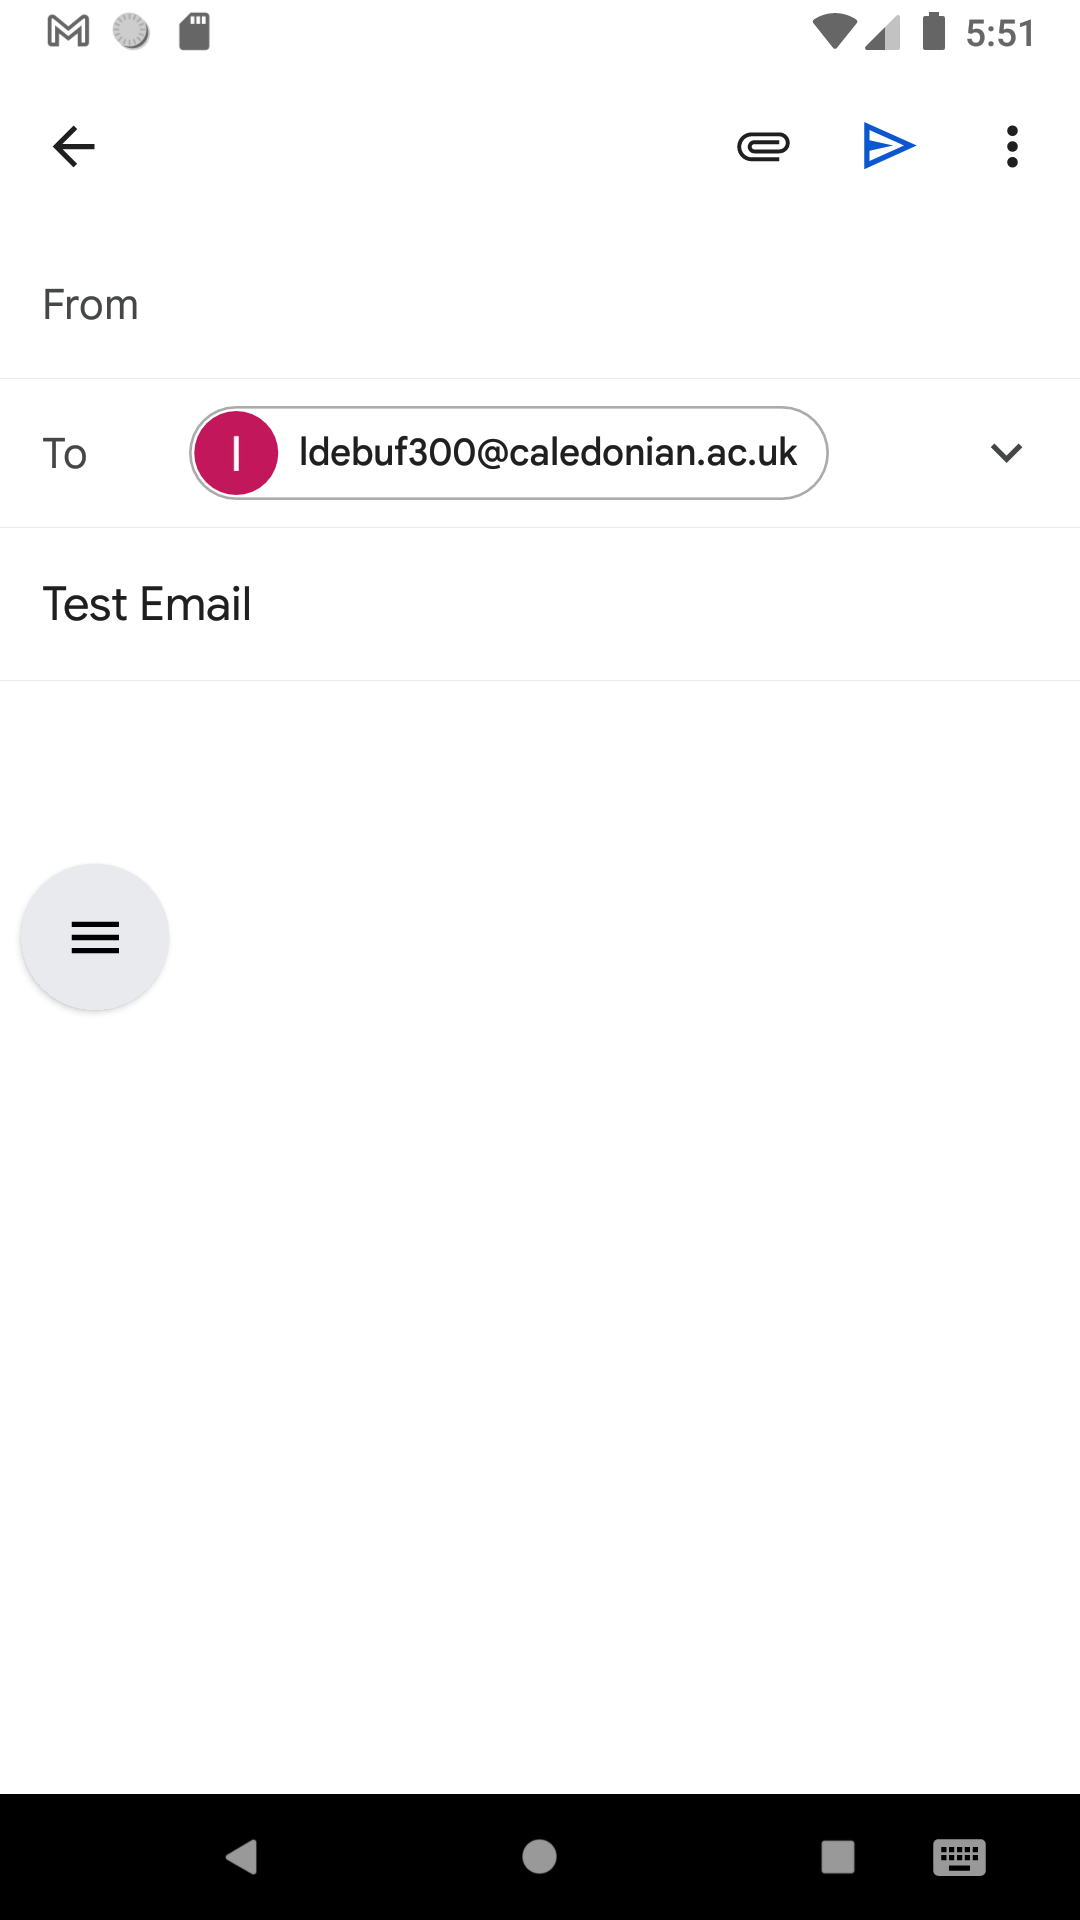
\includegraphics[width=0.45\linewidth]{implementation-figures/attach-before-noemail.png}
	\captionof{figure}{\textit{File attachment issue (email recipient has been hidden)}}
	\label{fig:file-attach-before}
\end{figure}

This required rewriting a majority of the function used to create the file. Instead of storing the file in internal storage, the file now had to be stored in a directory inside external storage, and
instead of using the FileOutputSteam class, which is better suited for multimedia files, the function now uses the FileWriter class, better suited for textual data 
. This rewritten code, and the successful attachment is shown below in code snippet \ref{lst:new-app-list-csv} and figure \ref{fig:file-attach-after}.

\begin{lstlisting}[language=Java, style=mystyle, caption={New implemention of writing the app list to a .csv file}, label=lst:new-app-list-csv]
private void generateFile(ArrayList<AppDetails> appDetails) {
    String fileName = "appDataDetails.csv";
    File exFileDir = this.getExternalFilesDir(Environment.DIRECTORY_DOCUMENTS);
    fileToEmail = new File (exFileDir, fileName);
    try {
        FileWriter fileWriter = new FileWriter(fileToEmail);
        for (int i = 0; i < appDetails.size(); i++) {
            fileWriter.append("\n").append(appDetails.get(i).appName).append("  |  ").append(appDetails.get(i).usageTime);
        }
        fileWriter.flush();
        fileWriter.close();
        Log.d("fileStuff", "File created successfully, located at: " + exFileDir);
    } catch (IOException e) {
        e.printStackTrace();
    }
}
\end{lstlisting}

\begin{figure}[H]
\centering
	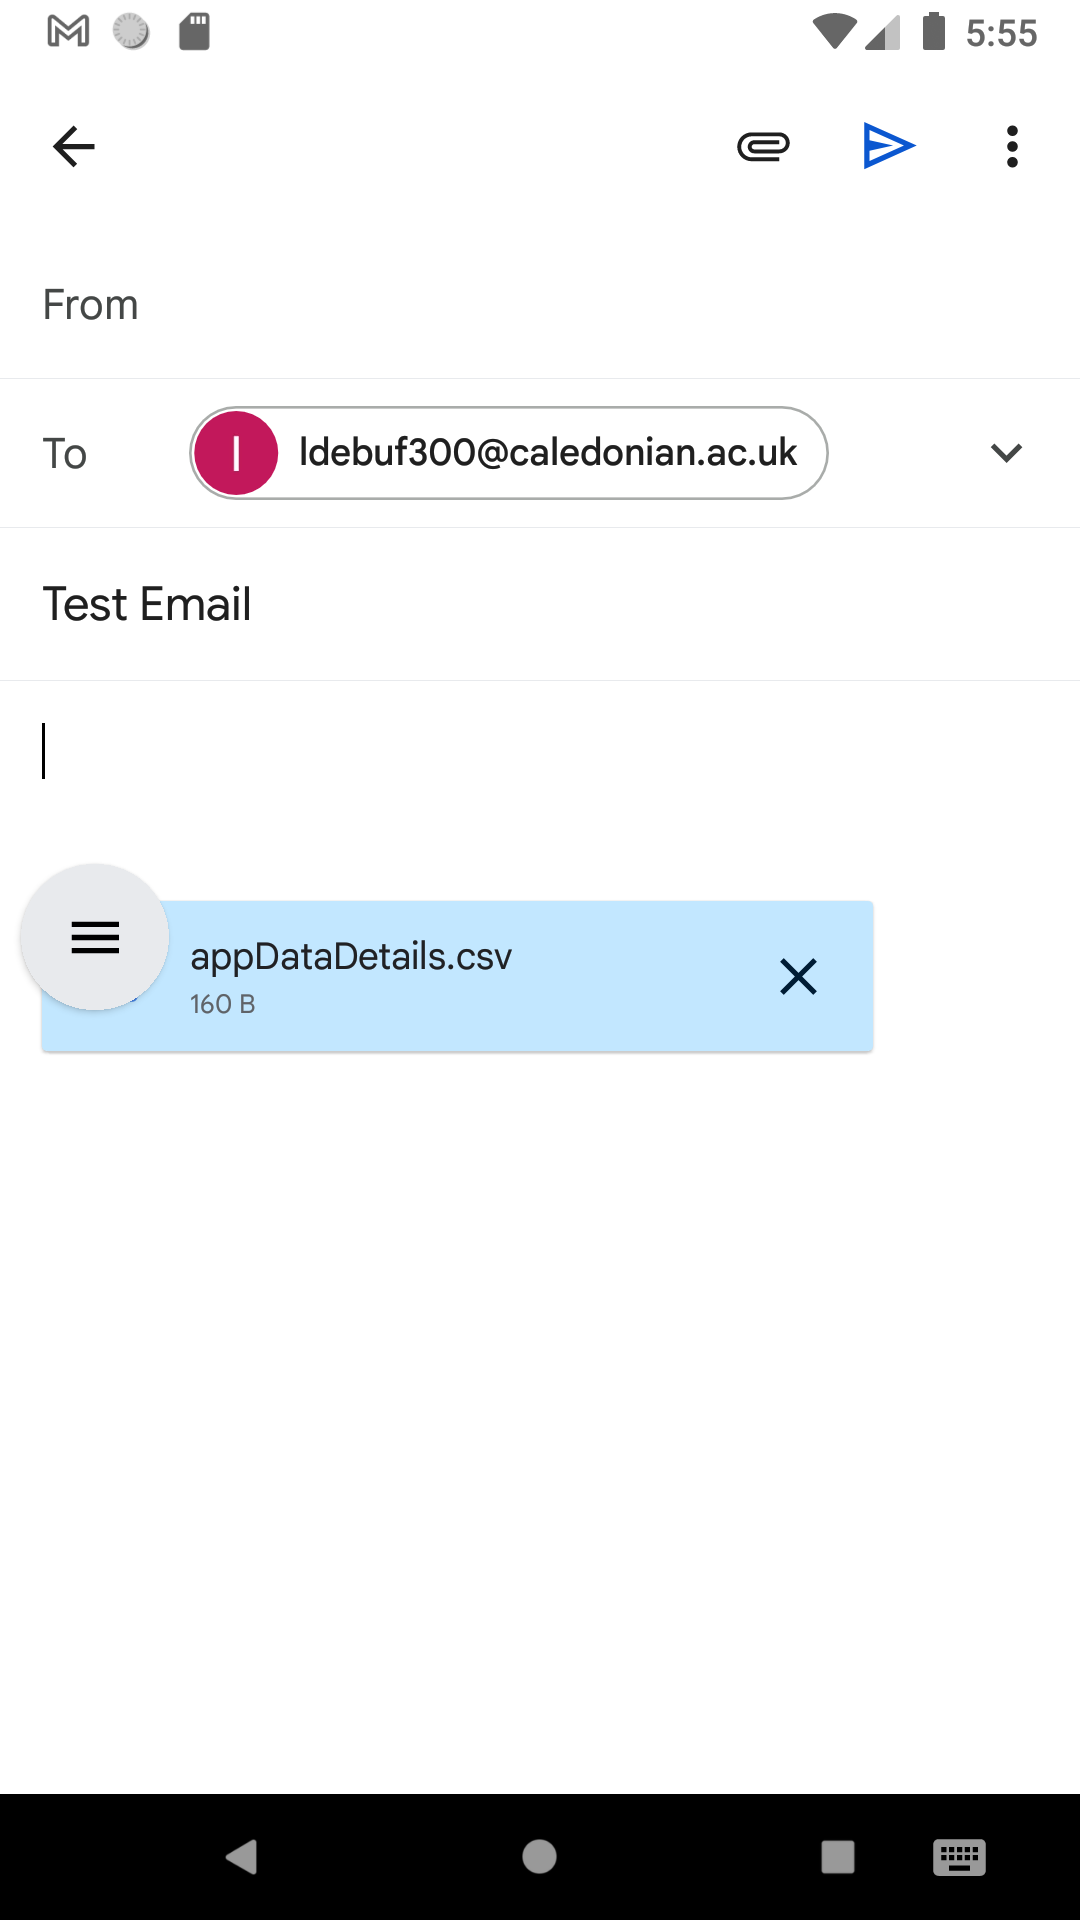
\includegraphics[width=0.45\linewidth]{implementation-figures/attach-after-noemail.png}
	\captionof{figure}{\textit{File attachment issue, now fixed (email recipient has been hidden)}}
	\label{fig:file-attach-after}
\end{figure}


\subsubsection{Req-1.3}
This branch is where the WDEP system from RT mentioned in section 2.3.3 of the literature review would see its continued implementation. The first step 
in implementing this was to create conditions the code can reach to show separate screens depending on if a user had seen an increase or decrease in their usage over the last week. This involved 
figuring out a way to store a users old usage time to compare, as the comparison would be used to send the user to correct set of screens.

\begin{lstlisting}[language=Java, style=mystyle, caption={Checking for usage increase / decrease}, label=lst:check-usage-increase]
long currentTime =  TimeUnit.MILLISECONDS.toSeconds(totalTime);
long oldTime = TimeUnit.MILLISECONDS.toSeconds(sharedPreferencesUsageTime.getLong("oldUsageTime", 0));

if (currentTime > oldTime) {
	Log.d("changeScreen1", "screen time has increased, different screen will appear here");
	screen_count = 10;
	screenCheck();
} else {
	Log.d("changeScreen2", "screen time has droppped, different screen will appear here");
	screen_count = 9;
	screenCheck();
}

sharedPreferencesNotiSent.edit().putBoolean("notiSent", false).apply();
sharedPreferencesUsageTime.edit().putLong("oldUsageTime", totalTime).apply();
\end{lstlisting}

Code snippet \ref{lst:check-usage-increase} shows the code used when the app checks for a usage increase or decrease, called once a week. currentTime is defined as the time value retrieved from the 
loadUsage() function (see code snippet \ref{lst:loadUsage}) while oldTime is the stored SharedPreference value of the variable, last updated from the prior week, when the function was last ran. The code will then 
swap to a corresponding screen depending on if there was an increase or decrease in usage. The code uses seconds as its time unit for debugging, while the final product makes use of hours 
instead. \newline

Because the user has the option of redefining their goal if they have seen a usage increase, the code for defining a goal had to be rewritten slightly. Shown below in code snippet 
\ref{lst:goal-definition-rewrite}, the code now checks if boolean value isRedefiningGoal is true, and if it is, updates the entered goal from the user. 

% isRedefiningGoal will be true if this 
% screen is reached from the screens used when receiving advice from the app.

\begin{lstlisting}[language=Java, style=mystyle, caption={Goal definintion screen, rewritten for requirement 1.3}, label=lst:goal-definition-rewrite]
 else if (isRedefiningGoal == true) {
	//TODO: possibly change paragraph text to make more sense given the context
	String oldGoal =  sharedPreferences.getString("goalEntry", "none");
	if (oldGoal.equals(goalEntryText)) {
		Toast.makeText(view.getContext(), "New goal cannot be identical to old goal", Toast.LENGTH_SHORT).show();
	}
	else {
		sharedPreferences.edit().putString("goalEntry", goalEntryText).apply();
		Toast.makeText(view.getContext(), "Goal has been updated to: " + goalEntryText, Toast.LENGTH_LONG).show();
		screen_count = 11;
		screenCheck();
		isRedefiningGoal = false;
	}
}
\end{lstlisting}

Code \ref{lst:pick-activities} below shows the code used for displaying a set of activities from the user. While the user activities are simply retrieved from the stored value using the 
SharedPreference API, the random hard-coded activities are retrieved from a separate string array file called strings.xml (see Appendix K), then two pseudorandom numbers are selected and are used to pick a random activity.,

% and 
% using those two numbers, two activities from the string array are picked at "random". All activities are the concatenated together and are shown to the user.

\begin{lstlisting}[language=Java, style=mystyle, caption={Code used for displaying activities to a user}, label=lst:pick-activities]
String[] activities = getResources().getStringArray(R.array.activities_array);
Random random = new Random();
int randomNumberOne = random.nextInt(activities.length - 1);
int randomNumberTwo = random.nextInt(activities.length - 1);

String randomActivityOne = activities[randomNumberOne];
String randomActivityTwo = activities[randomNumberTwo];

String userActivityOne = sharedPreferences.getString("activityOne", "none");
String userActivityTwo = sharedPreferences.getString("activityTwo", "none");
String userActivityThree = sharedPreferences.getString("activityThree", "none");

activitiesText.setText(userActivityOne + ", " + randomActivityOne + ", " + userActivityTwo + ", " + randomActivityTwo + ", " + userActivityThree);
\end{lstlisting}

\subsubsection{Req-1.2}
This branch was used to add

% the (at the time) final requirement for the app, that being 

the graph used for displaying the usage for the previous week to the user. While a wireframe diagram for this
screen was never created, re-using the idea of displaying the data in a list format was the decision made. \newline

The next step was establishing a method of storing the prior week's usage data to show the user. Because the code for creating a file already existed (see snippet \ref{lst:new-app-list-csv}), the 
code was simply adapted to create a separate .csv file if there was already an existing file. This adapted code can be seen below in code snippet \ref{lst:added-store-usage}

\begin{lstlisting}[language=Java, style=mystyle, caption={Adapted code for storing usage data}, label=lst:added-store-usage]
if (notiSent) {
	if (fileToEmail.exists()) {
		Log.d("fileExists", "file " + fileName + " already exists, creating file for previous week");
		String fileNamePrevWeek = "appDataDetailsPrev.csv";
		File exFileDirPrevWeek = this.getExternalFilesDir(Environment.DIRECTORY_DOCUMENTS);
		fileToEmail = new File (exFileDirPrevWeek, fileNamePrevWeek);
		//...
	}
}
\end{lstlisting}

The data from the .csv file then needs to be parsed properly to display it to the user, and this was achieved by using the external library OpenCSV abd the CSVReader class. The code shown below
in snippet \ref{lst:reading-csv-data} reads the file line-by-line, then adds it to an array list. Similar to what was achieved for requirement 1.1, this array list is then added to a 
ListView widget, then shown to the user. The full code block can be found in Appendix L.

\begin{lstlisting}[language=Java, style=mystyle, caption={Code used for reading .csv file data}, label=lst:reading-csv-data]
CSVReader csvReader = new CSVReaderBuilder(new FileReader(fileToShow)).withSkipLines(1).build();
String[] nextLine;
while ((nextLine = csvReader.readNext()) != null) {
	Log.d("prevWeek", nextLine[0]);
	previousWeekArrayList.add(nextLine[0]);
}
\end{lstlisting}

\subsubsection{Req 1.8 / Clean up}
This was the last branch created during development, and focused on getting the app ready for evaluation. This branch was also when the last requirement, requirement 1.8, was identified and implemented.
Implementing requirement 1.8 was conducted in a similar manner to requirement 1.3, that being to add a boolean variable, check if its true, perform input validation, then update 
the set of activities. A small snippet of the code used can be found below in code snippet \ref{lst:editing-activity}, but the full code block can be found in Appendix M.

\begin{lstlisting}[language=Java, style=mystyle, caption={Code added to activities definition code block}, label=lst:editing-activity]
 if (isEditingActivities == true) {
	String activityOne = sharedPreferences.getString("activityOne", "none");
	String activityTwo = sharedPreferences.getString("activityTwo", "none");
	String activityThree = sharedPreferences.getString("activityThree", "none");

	activityFieldOne.setText(activityOne);
	activityFieldTwo.setText(activityTwo);
	activityFieldThree.setText(activityThree);

}
//...
 /// if currently editing activities, send toast indicating change, then return to settings screen
if (isEditingActivities == true) {
	Toast.makeText(view.getContext(), "Activities have been updated", Toast.LENGTH_LONG).show();
	screen_count = 7;
	screenCheck();
	isEditingActivities = false;
	return;
}
\end{lstlisting}

Aside from adding this functionality, this branch replaced all of the placeholder text from previous branches with actual text, most of which was added to the strings.xml file mentioned in
section 3.6.6, added some extra functionality not explicitly noted in the SRS such as a help alert on the main screen, adjusted some of the time-sensitive values to reflect the intended
values, and added an app logo.

\newpage

\subsection{Testing}
At the end of each prototype iteration, Incremental Integration Testing was carried out to ensure that the requirements were implemented as intended according to how the requirement was
defined in the SRS. Incremental Integration Testing can be defined as testing components of a software system, one by one, adding components together until eventually the entire system
is being tested. As the nature of development involved creating a component based on the requirements specified, and only continuing once the component had been created to match the specification, 
this method of testing felt most appropriate. 


\begin{table}[H]
\centering
\resizebox{\textwidth}{!}{%
\begin{tabular}{@{}l|l|l|l|l|l@{}}
\toprule
\textbf{Test ID} & \textbf{Action}                                                                                                                  & \textbf{Expected Outcome}                                                                                                                                                                 & \textbf{Actual Outcome}                                                                                                                                                                   & \textbf{Evidence} & Assumptions / Context (If necessary) \\ \midrule
2.1              & \begin{tabular}[c]{@{}l@{}}User clicks on \\ “previous week” button \\ while no data for the\\ previous week exists\end{tabular} & \begin{tabular}[c]{@{}l@{}}A dialog pops up \\ explaining to the user \\ that no data for the \\ previous week currently \\ exists, and that \\ they should check back later\end{tabular} & \begin{tabular}[c]{@{}l@{}}A dialog pops up \\ explaining to the user \\ that no data for the \\ previous week currently \\ exists, and that \\ they should check back later\end{tabular} & Req\_2.1.webm     &                                      \\ \bottomrule
\end{tabular}%
}
\caption{Example of a test case}
\label{tab:test-case-example}
\end{table}

An example of how testing was carried out can be seen in Table \ref{tab:test-case-example}. The test case includes the test ID, mapped to match the requirement number, the 
action taken by a user that would trigger the component, the expected outcome of the test, the actual outcome of said test, evidence to show the 
outcome of the test, usually in the form of a screen recorded video or screen capture, and any additional context or assumptions needed to understand
the test case. A comprehensive list of the test cases and their results can be found in Appendix N. \newline


\newpage


\section{Evaluation \& Results Discussion}
This section provides details on the evaluation of the project in relation to the hypothesis stated in section 1.3, which was: \newline

\noindent\textit{The combination of usage tracking and intervention methods rooted in psychology within the created mobile 
application will help to address and reduce smartphone \& social media usage in young adults.} \newline

It also gives critical analysis and discussion of the results and findings from the evaluation, before drawing initial conclusions based on the
project hypothesis, research statement and objectives. Given the aforementioned hypothesis, the intention of the evaluation was to find if:

\begin{enumerate}
	\item The mobile phone usage from a participant decreased when comparing their usage from the start of the evaluation to the end.
	\item If there was a decrease in usage, was the PRI actually a contributing factor to it?
\end{enumerate}

\noindent When evaluating if the PRI met the project's hypothesis, objective, and research statement, a mixed-method approach was used. This approach can be defined as utilising quantitative and
qualitative methods in a study to obtain a deeper understanding of a phenomenon . The evaluation results are based off of the captured usage 
data from each participant, as well as the participant's own opinions of their experience using the PRI via a survey given at the end of the evaluation period. 

% While the obtained usage stats 
% will be the main focus, the results from the survey help to provide additional context and insights that quantitative data cannot easily do.

\subsection{PRI-Evaluation results}
Participants who agreed to take part in the evaluation were given the PRI for a period of 3 weeks. 

% Alongside this, they were given a Quick Start Guide that
% gave extensive details regarding using the app, as well as instructions on how to install the app and troubleshooting advice. 

Once they had set up the 
application, they were also asked to send their usage immediately afterwards. This was to use said usage stats as a baseline to compare the usage for the next three weeks.
While the data extracted initially shows the total usage which includes all apps used by a participant, the data was then further parsed by the author to analyse if
there was a shift in usage of social media apps. As discovered in section 2.2 in the literature review,  noted that people use their
smartphones for productivity reasons, and not just for social media. \newline

\begin{figure}[H]
\centering
	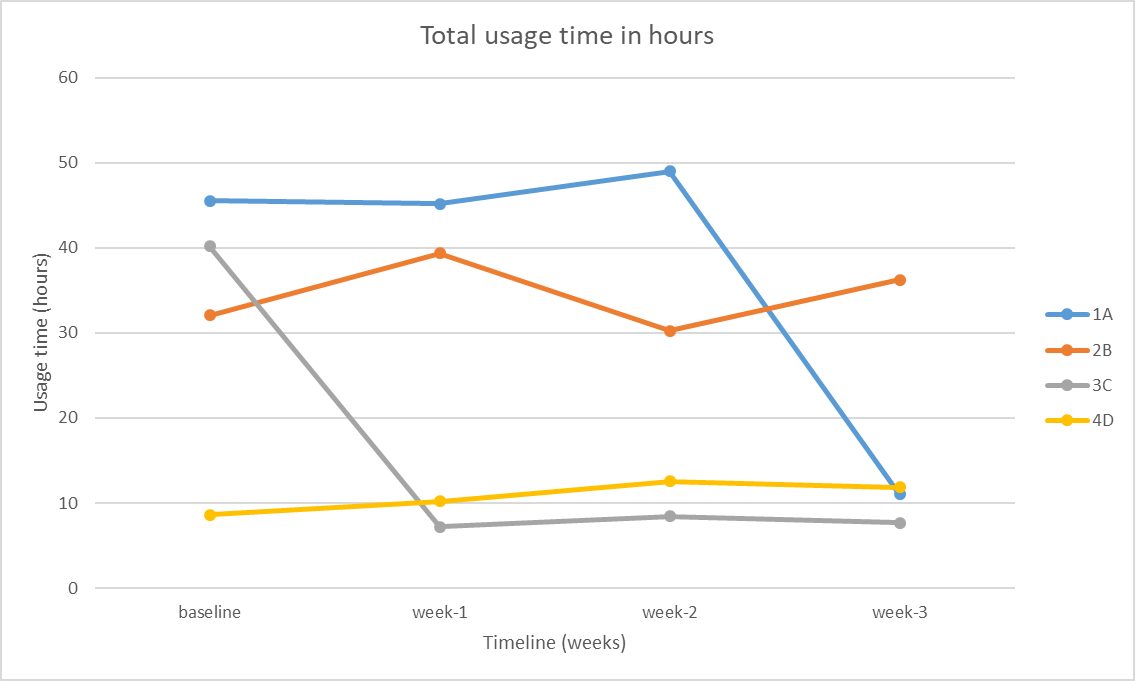
\includegraphics[width=1\linewidth]{eval-data-with-3c-basline-outlier.png}
	\captionof{figure}{\textit{Results from PRI evaluation}}
	\label{fig:eval-data-with-3c-basline-outlier}
\end{figure}

Figure \ref{fig:eval-data-with-3c-basline-outlier} shows the initial results from the evaluation, with the total usage from each participant. The x-axis shows the timeline of the evaluation period, from baseline to week 3. 
The y-axis shows the usage in hours. Table \ref{tab:3c-usage-sample} shows a sample of the usage data captured, showing the name of the app package (a unique identifier for an android app), the usage time
for the app, and the percentage of the usage time. 

\begin{table}[H]
\centering
\begin{tabular}{@{}|l|l|l|@{}}
\toprule
android     & 24:50:00 & 61\% \\ \midrule
maps        & 04:18    & 10\% \\ \midrule
One UI Home & 01:21    & 3\%  \\ \bottomrule
\end{tabular}%
\caption{Sample of usage data from participant 3C.}
\label{tab:3c-usage-sample}
\end{table}

% Within the dataset, an outlier was detected within the baseline data for participant 3C. 

Seen above in table \ref{tab:3c-usage-sample}, the "android" 
package, which refers to the android home screen, takes up over 24 hours of usage time. Seeing as this may be unrealistic for a typical user, the decision was
made to leave out the usage time for "android". Figure \ref{fig:eval-data-without-3c-basline-outlier} below shows the chart 
without the outlier data.

\begin{figure}[H]
\centering
	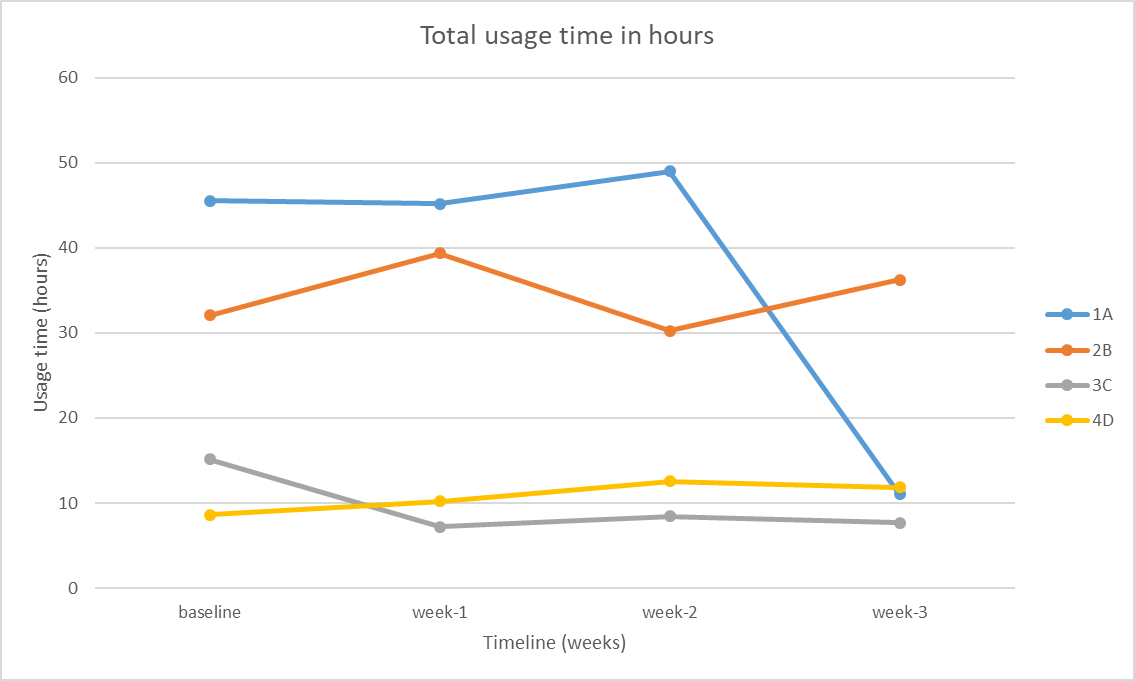
\includegraphics[width=1\linewidth]{eval-data-no-3c-basline-outlier.png}
	\captionof{figure}{\textit{Results from PRI evaluation, without the outlier data}}
	\label{fig:eval-data-without-3c-basline-outlier}
\end{figure}

1A's usage is relatively consistent between baseline and week-2, but takes a substantial
drop in week-3. 2B's usage fluctuates a lot throughout the timeframe, initially rising before falling again, and then settling in the middle for week-3. 3C's usage does take a drop overall 
when comparing baseline to week-3, and remains under 10 hours for the remainder of the evaluation period after the baseline data. 4D's usage experiences a slight increase before dropping 
slightly, though experiences an overall increase.  

\begin{figure}[H]
\centering
	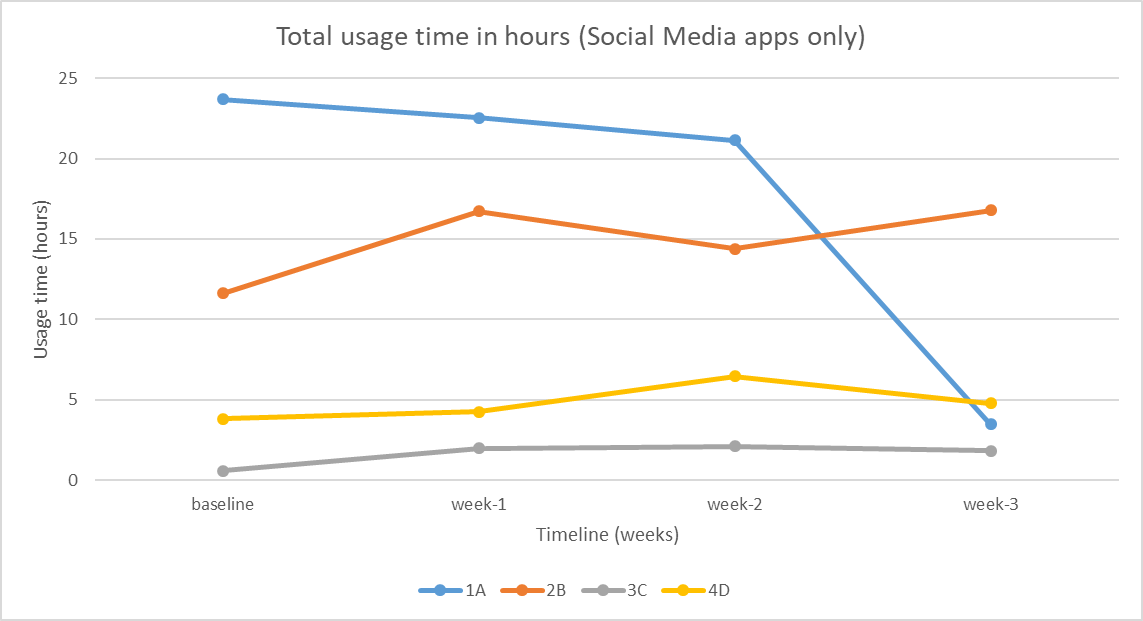
\includegraphics[width=1\linewidth]{eval-data-social-media-only.png}
	\captionof{figure}{\textit{Results from PRI evaluation, only showing social media usage}}
	\label{fig:eval-data-social-media}
\end{figure}

Figure \ref{fig:eval-data-social-media} shows the same graph as figure \ref{fig:eval-data-without-3c-basline-outlier}, but only including social media usage from each participant. 
While the graph is relatively the same, there are some differences. For example, unlike the total usage, 1A's social media usage never increases, rather, takes a small decline 
instead. 4D's social media usage starts, and remains quite low, though does take a small increase in week-1 before levelling out by the later weeks.

\subsection{Post-Evaluation survey results}
Part of using a mixed-method approach involves collected qualitative data, which can be defined as written text, images, audio 
recordings to name a few . While the data from the previous section are an important piece
of the evaluation as a whole, getting this kind of data helps to understand the thoughts and feelings from participants, and help in understanding
and contextualising the behaviours represented in the previous section.\newline

At the end of the evaluation testing period, participants were sent a survey to fill out. This survey gave participants the opportunity to express their
opinions on the evaluation period, with the survey including a variety of multiple choice and open-ended questions. Two question
sets were provided, one focusing on how the participant felt after using the app, and the other focusing on the overall functionality of the app. 

% move to appendix maybe
% The number of 
% respondents matched the number of participants who took part in the evaluation, that being 4. Note that because the open-ended questions were optional, not all 
% participants provided a response to them.\newline

\begin{figure}[H]
\centering
	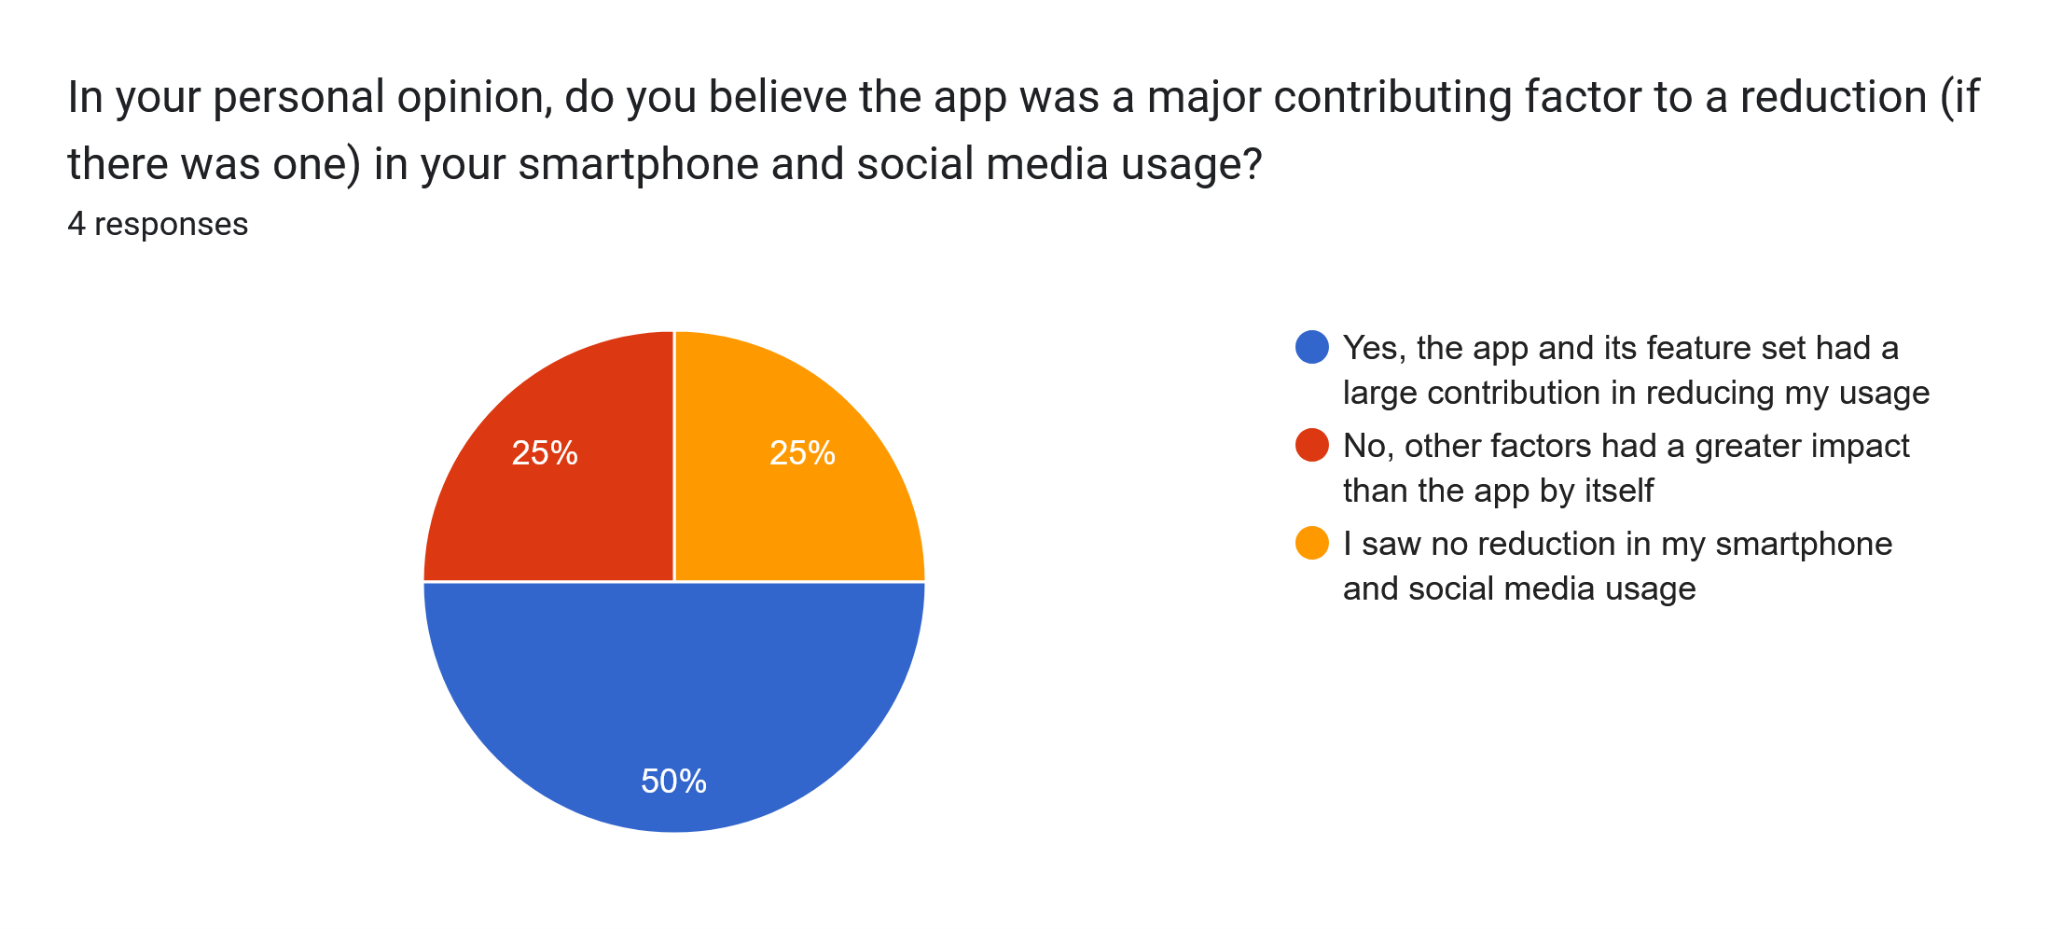
\includegraphics[width=1\linewidth]{Q3-evaluation-survey.png}
	\captionof{figure}{\textit{Results from question 3 from the post-evaluation survey}}
	\label{fig:question3surveyresults}
\end{figure}

A complete collection of the questions and responses can be found in Appendix O, however, the sentiment derived from 
the results of QS1 show that users felt more informed about their usage after using the app, and on average, users felt as if the app
implemented the WDEP system to a good degree. As demonstrated in figure \ref{fig:question3surveyresults}, only two of the respondents felt that the app contributed to their
lowered usage, with one respondent feeling as if other factors had a bigger impact than the app by itself, and the other feeling like there wasn't any
reduction in their usage. When asked to provide a reason to their choice, one respondent said in reference to the app lowering their usage:\newline

\textit{"It works pretty well! I feel as if seeing your values and hobbies increases motivation to not chase social media and other applications"}\newline

Another response, in reference to the participant not seeing a usage drop, stated:\newline

\textit{"At this time of year as a student based outside the city of my university I was regularly on my device to check on my classes and assignments"}\newline


% may be cut, not too related to the evaluation intention

% \begin{figure}[H]
% \centering
% 	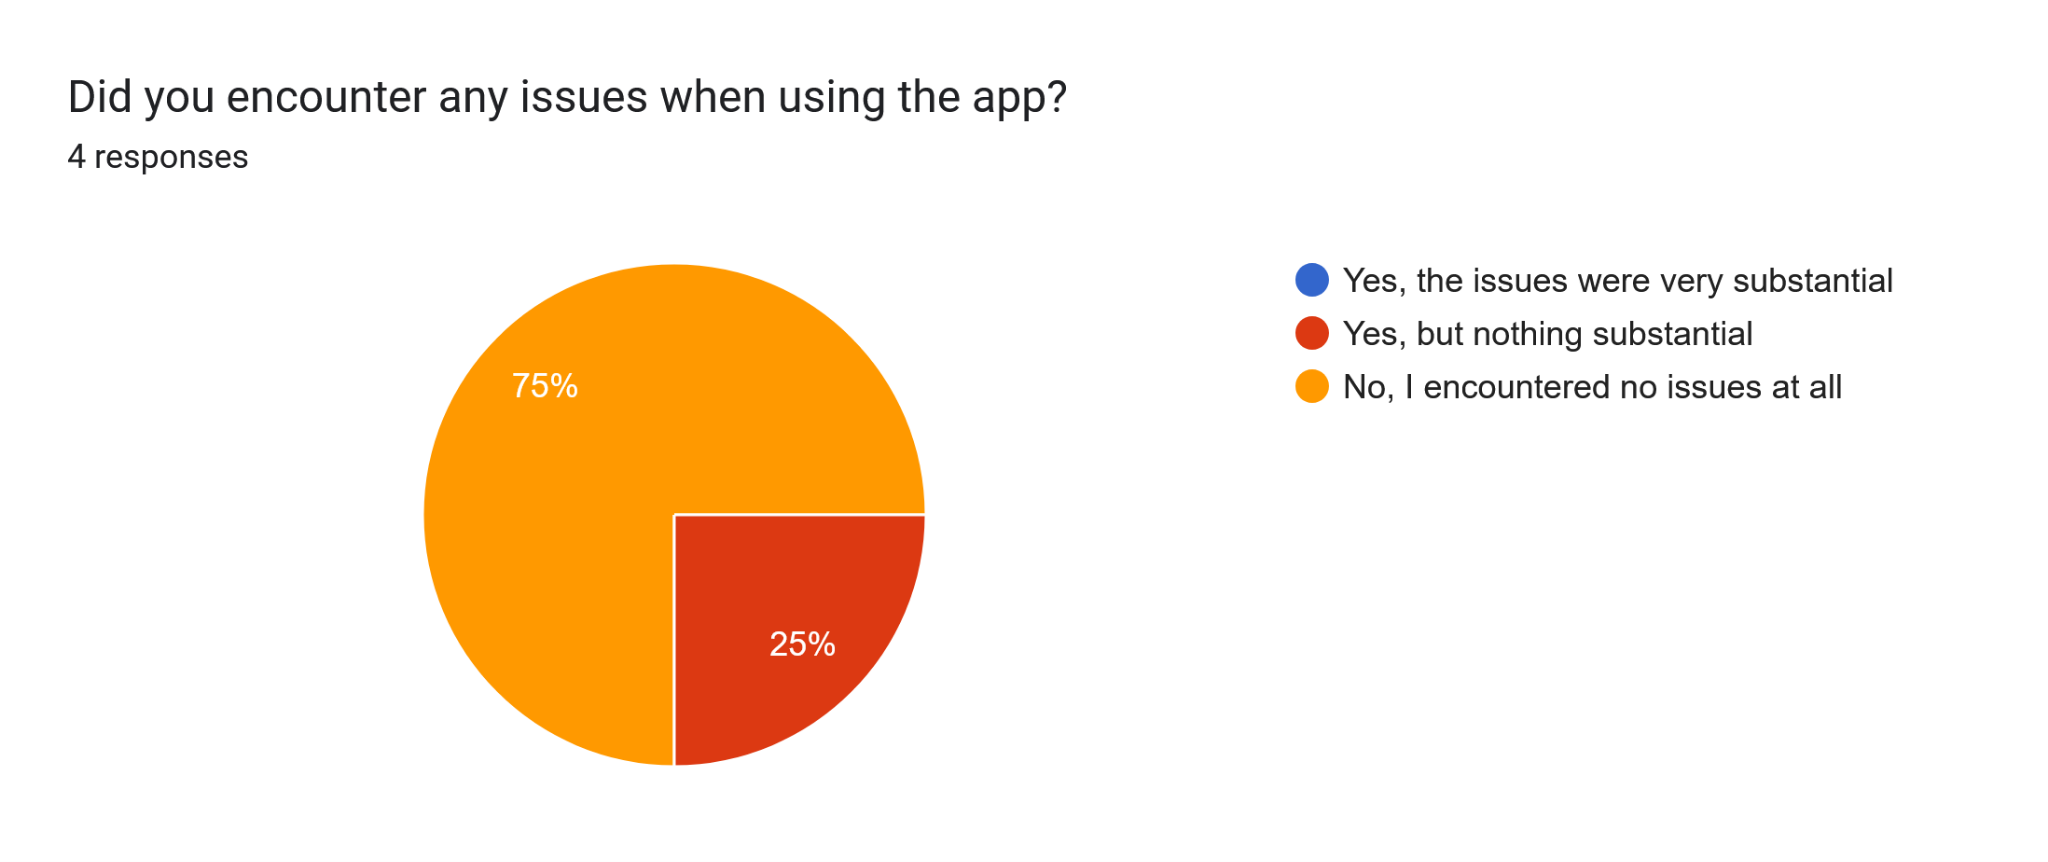
\includegraphics[width=1\linewidth]{Q11-evaluation-survey.png}
% 	\captionof{figure}{\textit{Results from question 11 from the post-evaluation survey}}
% 	\label{fig:question11surveyresults}
% \end{figure}

% The responses to QS2 show that respondents generally had a positive experience using the app, with no participant experiencing any substantial issues. One
% participant did however note one smaller issue, stating:\newline

% \textit{"I find that the email prompt would be better and easier to understand is [sic] it was titled "report" or something similar"}\newline

% Participants were asked if the app experience was better than existing apps that provided similar functionality, while 3 of the participants stated that they haven't
% used apps similar to the PRI, one participant disagreed that the app experience was better than existing apps. When asked to provide a follow-up stating what the PRI
% could take note of, they stated:\newline

% \textit{"an app called Screen Zen which gives more options to limit screen usage."}\newline

% When asked to provide suggestions on how the app could be improved, one response suggested increasing the notification frequency from being sent on a weekly basis
% to a daily basis, while another suggested showing how the app usage for specific apps have changed between weeks. 

At the end, participants were finally asked to
provide any closing thoughts regarding their experience, and while only one participant gave a response, they stated that they believe the app is a step in the 
right direction in addressing SA and SMA.


\subsection{Discussion}

% maybe remove? kinda hesitant
% The intention of the evaluation was to find if the PRI satisfies the project's hypothesis, and this was done by collecting quantitative data in the form of usage data captured
% from each participant and qualitative data in the form of a survey given to participants at the end of the evaluation period, where participants could provide their opinions on the
% current state of the PRI. \newline

The quantitative data initially revealed that only three participants experienced a drop in smartphone usage at some point during the evaluation, and only two 
of the participants' usage was lower by the end of the evaluation period. Discussed in section 2.2, discussed how smartphones can be used 
for productivity and not exclusively for social media, so the data was reanalysed to look exclusively at social media apps, and found the results were largely the same between all participants when compared to
the initial set of data.\newline

The qualitative data revealed that participants found themselves informed about their smartphone and/or social media usage. This was another talking point from 
, as it was discussed that intervention apps don't provide an opportunity for users to reflect and learn about SA and SMA. Not only this,
the data revealed that some participants attributed the PRI as a factor in their reduction in smartphone and social media usage, all participants in their opinion felt that the app
helped them achieve the goal they set out with one participant stating the app is a 
step in the right direction when addressing the issue of SA and SMA.\newline

Given this, the PRI can be considered somewhat successful in meeting the project's hypothesis. This is because The quantitative data provided mixed results when it came to reducing the 
usage of all participants in both a general sense and specifically with social media, however, the qualitative data provided a juxtaposition, with some participants believing the app was 
helpful in reducing their usage, most saying they would recommend the app to a friend, and all participants believing the app helped them achieve their goals (see Appendix O).


\newpage


\section{Legal, Social, Ethical, and Professional Issues}
This section will provide commentary on Legal, Social, Ethical, and Professional (LSEP) issues the project dealt with over its lifespan.
Within the Social Issues section, it will also provide additional commentary and reflection on the Sustainable Development Goals (SDGs)
the project has aligned itself.

\subsection{Legal Issues}
While the project didn't encounter any issues related to copyright, the project did have to deal with issues to data protection, particularly in
relation to the Data Protection Act 2018 and the UK General Data Protection Regulation, two laws that relate to protecting the personal data of
individuals . \newline

Any data taken from participants was ensured to be compliant under the Data Protection Act 2018. When ensuring the protection of 
user data, all information was kept in a local folder on the author's PC at his home, as well as on an external USB.\newline

When a human participant was involved at any stage of the project, it was clearly outlined to them what kind of data would be collected and
processed. For example, during the evaluation stage, when the user opens the app for the first time, the user is given full clarity on the
purpose of them using the app, as well as what kinds of data the app would be collecting. At no point does the app capture any personally
identifiable information from a participant. 

\subsection{Social Issues}
The projects primary subject matter involved addressing the issue of addiction pertaining to social media and smartphones. When discussing
the topic of addiction, it's important that the issue is addressed in a non-stigmatizing manner and with respect to those who may be dealing
with such issues . Throughout the report, the issue of addiction has been discussed in a way that
doesn't stigmatize those who may be dealing with, or have dealt with such issues. As well as this, at no point within the report does the author 
claim the PRI to be a treatment for the issue of SA \& SMA, rather, as a teaching opportunity for someone to learn about the issue.

\subsubsection{Sustainable Development Goals}
This project has aligned itself with Sustainable Development Goals 3 and 4. Below are the definitions provided by the United Nations:

\begin{itemize}
	\item Ensure healthy lives and promote well-being for all at all ages .
	\item Ensure inclusive and equitable quality education and promote lifelong learning opportunities for all .
\end{itemize}

Target 3.4 for SDG 3 states that by 2030, it should:\newline

\textit{...reduce by one third premature mortality from non-communicable diseases through prevention and treatment and promote 
mental health and well-being} .\newline

The project's intention from the very beginning was to encourage healthier smartphone and social media usage. It attempts to achieve this by encouraging the user to partake in activities
away from their smartphone and set goals for themselves that they can achieve away from their smartphone and social media. \newline

In relation to goal 4, a key component of the app is making the user aware of their habits, and what they can do to lower their smartphone and social media usage, should it be at a high level. This is
also helped through the use of the WDEP system introduced by Reality Therapy, whose system intrinsically includes learning opportunities through self-evaluation. This teaching aspect was also a 
component that was intended to be included following the literature review. \newline

Through the promotion of better smartphone habits, and through provided opportunities for the user to learn about their smartphone habits, the author believes the project correctly aligns with
these two goals.

\subsection{Ethical Issues}
As previously mentioned when discussing
the project's primary objectives in section 1.2.2, for conduction the evaluation, human participants were required to carry out said
evaluation as intended, which involved collecting app usage data from participants, as well as responses from the post-evaluation survey.
 This aspect by itself already constitutes as an ethical issue, given the use of human participants for a project
of this nature raises concerns regarding the autonomy and well-being of participants,
, but this specific use of human participants brings forth the issue of data collection. \newline

Similarly, during the requirements analysis stage of the project's execution, a survey was distributed, and 1-to-1 interviews were 
conducted. Given the use of software tools to carry out these parts of the project, this raises issues with data protection, informed 
consent, and the privacy of participants . Dealing with such issues required taking different precautions 
at each step. When ensuring the privacy of participants at any stage, identifying information was either redacted, anonymised, or not 
collected at all. \newline

When conducting user interviews and the evaluation, participants were given a consent form to sign before taking part in anything related 
to the project, and before taking part in any survey, participants were asked to provide informed consent to take part and were given as 
much information as possible, something which was noted as an issue by . \newline

To conduct any part of the project where human participants are required, ethical approval was required to be granted 
prior to conducting any part of it. All the details written about previously were mentioned within the ethics form, alongside reasonable 
justification, and ethical approval was granted.

The code used for the PRI sources a small sample of the code from an external sample project as a basis for loading, and showing the usage for
a user. This code has been attributed to the respective author in both the source code for the PRI, as well as the report in section 3.5.1, and
within Appendix I.

\subsection{Professional Issues}
Following the completion of this project, there are a few aspects that have been reflected on that the author believes have undertaken well, and
others the author wishes would've been undertaken differently. Section 3.3 details the SDLC used during the project's execution, and 
how there was a change in SDLC midway through the project. Instead of this conducting this change midway through the project, this change 
could've occurred before any work was carried out, or could've been prevented altogether if deeper research was conducted at that stage. \newline

The author believes that issues related to transparency were handled well. Information related to how the data of participants would be used, as
well what their involvement would and wouldn't entail were communicated at every possible step, and participants were offered the choice of 
opting out of any project-related activity at any given time, without notice. Participants were told to forward any issues or questions they
may have to the author, showing a level of accountability and responsibility taken by the author. 


\newpage
\section{Conclusions and Further Work}

\subsection{Summary}
Over the past fifteen years, smartphones and social media have been quickly integrated into wider society. Both of them serve as an important component of everyday life for a large number of 
people and have helped connect people with each other from around the globe on a never-before-seen scale. With this, however, the issue of individuals developing an overdependence on such 
technology has become a prominent talking point when discussing them. Subsequently, studies have been carried out analysing the issue, its causes, its effects on one's health, and potential 
solutions, one of which being intervention apps that attempt to help users lower their usage, and another being the use of psychological methods. With that being said, a gap of intervention apps
that deal with the aforementioned issue was found. The primary aim of the project was to carry out the research statement, being: \newline

\textbf{To create a mobile application that integrates psychological intervention methods alongside usage tracking technologies to help address smartphone and social media addiction} \newline

A literature review was carried out to investigate existing applications that use psychological intervention methods when addressing related issues, how SA and SMA are contextualized within 
existing apps and the issues they raise, existing psychological frameworks that can be integrated into a mobile application, and methods to track a user's app usage. \newline

Following the findings from the literature review, an effort to create a mobile application that used usage tracking technologies and psychological intervention methods while following a 
”develop and test” approach began. A development lifecycle was chosen, initially being an agile methodology before switching to a hybrid methodology.Thereafter, an analysis of the requirements 
necessary for the app to function as intended was undertaken, as well as picking a psychological intervention and usage tracking method, those being Reality Therapy and using the
android.app.usage package, respectively. Flowchart design diagrams showing the app flow for each requirement and UI wireframes that depict how each app screen should look were then created. 
After this, the process of coding the app based on the information created and obtained began. After each iteration, testing was performed to ensure the app worked without issue. Finally, an 
evaluation with multiple participants took place where they used the app over a three-week span and sent their usage data for further analysis at one week intervals, before answering a survey 
at the end of the three-week period.

\subsection{Results}
To reiterate what was stated in section 4; based off of the hypothesis, the intention of the evaluation was to find out if:

\begin{enumerate}
	\item The mobile phone usage from a participant decreased when comparing their usage from the start of the evaluation to the end.
	\item If there was a decrease in usage, was the PRI actually a contributing factor to it?
\end{enumerate}

\subsubsection{Was there a decrease in usage?}
The quantitative data gathered and presented in section 4.1 reveal that only two of the four participants' usage decreased overall when comparing their usage at the start to the end of 
the evaluation period, with this result staying consistent when only social media apps are included in the dataset. Therefore, this first point is proven to be plausible, or somewhat true.

\subsubsection{Was the PRI a factor in a reduction in usage?}
The qualitative data gathered and presented in section 4.2 reveal that participants who experienced a usage drop at some point during the evaluation period positively attributed the app to be 
a significant factor in a reduction in that usage, and carry the opinion that the app helped them achieve their set goal. Therefore, this second point is proven to be true beyond a reasonable
doubt.

\subsubsection{Conclusion}
To conclude, the PRI and project as a whole successfully satisfies the research statement and project hypothesis, yet only does so to an extent. The project does indeed create a mobile app that 
uses psychological intervention methods with usage tracking technologies to address the issue of SA and SMA, and has also shown to reduce the smartphone usage in young adults. However, from the 
results of the evaluation, the PRI only reduced the smartphone and social media usage in two of the four participants. This is juxtaposed from the opinions from the participants themselves, who 
believe that the app played a significant role in reducing their smartphone and social media usage.

\subsection{Limitations \& Project Critique}
Despite proving the research statement and project hypothesis to be true, the project is limited in some regards. A limitation of the project was the use of only one 
psychological intervention method. The project only uses a single concept from a single psychological framework, that being the WDEP system from Reality Therapy. The 
decision to use a single intervention method from a single framework was made to limit scope creep and to keep development as simple as possible. Within the intro and
literature review, CBT is referenced as a psychological framework that has seen use and success in apps similar to the one made for the project, so, integrating
frameworks such as ones seen in CBT would be an area of improvement. \newline

Although not an issue for the current iteration of the project, from September of 2026 onwards, apps to be installed on Android devices in certain regions will have to be from verified Android 
developers . This means that future research that involves evaluating an app on a real device with human participants will require a researcher to be an Android verified developer, or go through 
the process of side-loading the app. \newline

The project was also limited during the evaluation phase due to the number of participants involved. While the intention was to gather ten participants for the evaluation, only four participants 
were gathered. The reasoning behind this lacklustre turnout may be due to poor recruiting efforts when gathering participants, as recruiting efforts were limited to a small group of people. 
Should a project of this calibre be attempted again, promoting the evaluation to a wider group of individuals, perhaps in physical areas such as university campuses, may prove to be an effective 
method of gathering participants.

\subsection{Further Work}
When it comes to other work this project could potentially influence, investigating what psychological framework between CBT, RT, or another psychological framework 
in an app of this nature, and which one proves to be more beneficial from a quantitative and qualitative standpoint could an area that could use further coverage, and this 
could influence further use of a framework, establishing it as a standard when addressing the issue of SA and SMA. \newline

On the contrary, and as alluded to in the previous section, future work could benefit from integrating more than one psychological intervention method, such as CBT, and 
its various methods mentioned in the literature review such as behavioural activation, cognitive restructuring, and problem solving. From a technical standpoint, using
app restriction functionality with usage tracking alongside either, or both psychological frameworks could shed further light on this topic area.\newline

Expanding the target audience to include other age groups such as adolescents or older individuals could prove beneficial when evaluating apps of this nature in future 
studies, as it could provide deeper insights into the smartphone and social media usage habits of those groups.




\newpage
\addcontentsline{toc}{section}{References}
\printbibliography

\newpage
\end{document}